\chapter{Synapse Structure}

Common facts:
\label{sec:synapse-number-per-neuron}
\begin{verbatim}
rate of neuron growths at early pregnancy = 250,000 neurons/minute
length of spiny terminals of Purkinje cells = 40,700 micron
# spines on Purkinje cell dendritic branchlet = 61,000
# Purkinje cells = 15-26 million
# synapses made on Purkinje cells = 100,000 - 200,000

# synapses made on a 'typical' neuron = 1,000 - 10,000

\end{verbatim}
% Each neuron has as many as 15,000 connections with neighboring neurons.
% \textcolor{red}{In general, a typical neuron has about 8,200 synapses}. 
And an adult brain (CNS) has totally about 100-500 trillion synapses. 
\url{https://faculty.washington.edu/chudler/facts.html}

The discussion about different types of synapse is given in
Sect.\ref{sec:synapse}.
\begin{itemize}
  \item axon-axon
  \item axon-dendrite
  \item dendrite-dendrite
  \item axon-soma
\end{itemize}

The vast majority of synaptic inputs impinge on the dendrites rather than the
soma or the axon.
Synapses themselves are plastic (Sect.\ref{sec:synaptic_plasticity}), with the
plasticity being governed by the temporal patterns of presynaptic and
postsynaptic activities - a process underlying learning and memory
\ref{sec:synaptic_plasticity_model}.
The activity at the posynaptic itself is in turn determined by the properties
(volume, size, channel densities) s of the dendritic arbor itself, implying that
the dendrites must in part determine the rules that govern synaptic plasticity.

\section{Synapse}
\label{sec:synapse}

Even though Cajal had suggested that there is no cytoplasmic continuity between
neurons, the experimental evidences were not available until synapses was found
by using electron microscopy (EM) in 1950s. Sir Charles Scott Sherrington and
colleagues coined this term {\bf synapse} from the Greek ``syn-'' (``together'')
and ``haptein'' (``to clasp'') in their book ``A Textbook of Physiology, part three:
The Central Nervous System'' in 1897.

These synapses are responsible for the propagation of information from one
neuron to the next.  Interestingly, information transmission in the nervous
system is partly electrical and partly chemical. When the action potential
(which is electrical signal) reaches the synapse, this leads to vesicle fusion
and subsequent release of chemical signals (neurotransmitters) which induce
channel gating in the neighboring cell with which it has formed the synapse.    
 

\subsection{Numbers}

The total number of such synapses in the human brain has been vaguely stated to
be in the range of $10^{13}-10^{15}$ (about $10^{13}$ in human cortex, and
$10^{15}$ in human connectome - the network of elements and connections forming
the human brain) (Pakkenberg et al., 2003), with every cubic millimeter of
cerebral cortex having about a billion such synapses (BNID 109245).
\url{http://book.bionumbers.org/how-big-is-a-synapse/}

%http://bionumbers.hms.harvard.edu/bionumber.aspx?s=n&id=100693&ver=5
% Pakkenberg B, Gundersen HJ, Mortensen EL, Lauritzen MJ, Jeune B, Regeur L, West
% MJ, Schwartz TW. [The normal brain: a new knowledge in different fields] Ugeskr
% Laeger. 1997 Feb 3 159(6):723-7. AND Pakkenberg B, Pelvig D, Marner L, Bundgaard
% MJ, Gundersen HJ, Nyengaard JR, Regeur L. Aging and the human neocortex. Exp
% Gerontol. 2003 Jan-Feb38(1-2):95-9.   
  


% The word 'synapse' was coined by Sir Charles Sherrington in 1897 to denote
% normal anatomical relations between contiguous neurons, and they recognized
% synapse as a discontinuous intercellular junction.
\subsection{Pre- and Post-}

A synapse has pre-synaptic and post-synaptic elements
\begin{itemize}
  \item pre-synaptic element: Sect.\ref{sec:axon-terminal}
    
  \item post-synaptic element: Sect.\ref{sec:spine}
\end{itemize}

The small gap between the pre-synaptic region and post-synaptic region is called
{\bf synaptic cleft} (junctional cleft) - Sect.\ref{sec:synaptic-cleft}, as
shown in Fig.\ref{fig:terminal_button}\footnote{http://www.frca.co.uk/article.aspx?articleid=100618}.
% The post-synaptic region is not flat, but is heavily folded.

\subsection{Size of a synaptic cleft}
\label{sec:synaptic-cleft}

The tiny space betwen the axonal terminal and post-synaptic side (which can be
either the dendritic shaft or a dendritic spin) is called the {\bf synaptic
cleft}, which has different sizes, Fig.\ref{fig:synapse-size}.

The size also depends on different kinds of synapses
\begin{enumerate}
  \item neuromuscular synapse - Sect.\ref{sec:neuromuscular-junction}
  
  \item calyx of Held synapse - Sect.\ref{sec:calyx-of-Held-synapse}
  
  \item 
  
  average volume of the synaptic cleft: $0.76 \times 10^{-3} \mum^3$, which was
  calculated from active zone size and PSD areas.
  If we consider the effective diffusion volume to which the neurotransmitter
  has rapid access, then the value could be very much larger. The diffusion
  volume for a single active zone in the brain was found to be about 50x
  higher, i.e. $44 \times 10^{-3} \mum^3$.
  
  
  
\end{enumerate}


\begin{figure}[hbt]
  \centerline{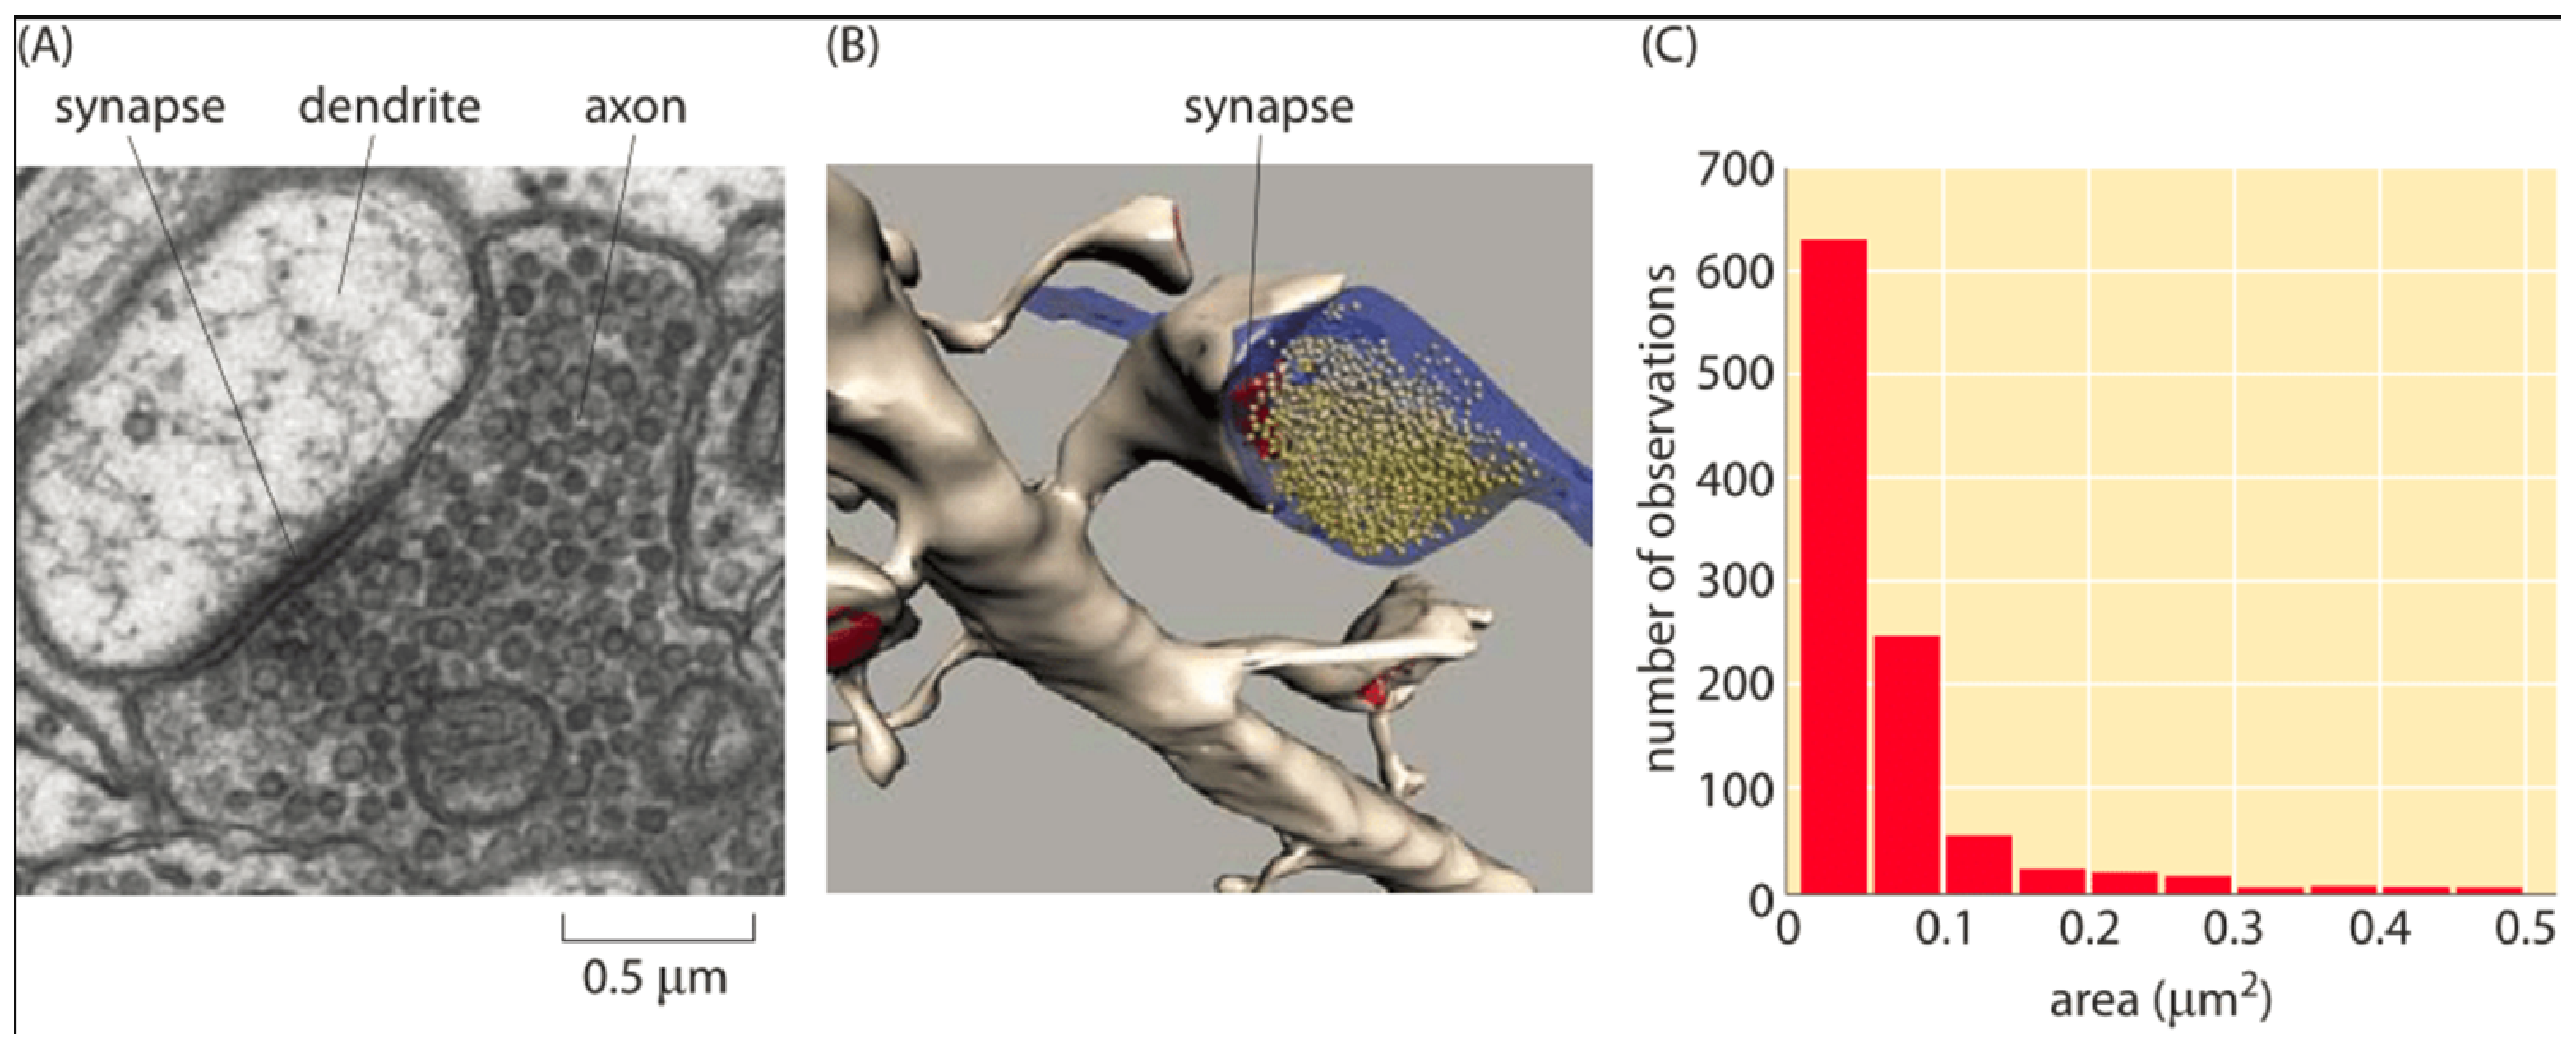
\includegraphics[height=3cm,
    angle=0]{./images/synapse-size.eps}}
  \caption{Size of synapses in the brain. (A) Electron microscopy image of a
  synapse between an axon and a dendrite. (B) Reconstruction of a synapse like
  that shown in (A) illustrating the synaptic vesicles. (C) Distribution of
  synapse sizes as measured using electron microscopy. (Figures courtesy of
  Linnaea Ostroff) }
\label{fig:synapse-size}
\end{figure}


\url{http://book.bionumbers.org/how-big-is-a-synapse/}


\subsection{Classification 1: chemical + electrical synapse}

{\bf SYNAPSE CLASSIFICATION}: In general, there are 2 types of
synapses in CNS
\footnote{\url{http://www.ncbi.nlm.nih.gov/books/bv.fcgi?rid=neurosci.section.318}}:
\begin{itemize}
\item {\it chemical synapses}: with {\it synaptic cleft} within
  20-40nm.
  \textcolor{red}{By default, i.e. without a quantifier, synapses
    means ``chemical synapses''}.

Most synapses are uni-direction (signals are transmitted from pre-synaptic to
post-synaptic), except {\it electrical synapses}.

\item {\it electrical synapses}: with synaptic cleft about 3.5nm which
  is extremely closed that makes the two cells actually linked together by an
  intercellular channel (specialization) called {\it gap junction}
  (Sect.\ref{sec:gap-junction}). The short distance allows the signals to be
  transmitted in a passive manner, i.e. much faster in here than in chemical
  synapses. More important, it's bi-direction.
  
\end{itemize}
There is a third type: {\it immunological synapses}: between
antigen-presenting cell and lymphocyte (not occur in the CNS).

\subsection{Chemical synapse classification: symmetric + asymmetric}
\label{sec:synapse-symmetric}
\label{sec:synapse-asymmetric}

EM studies in the cortex have revealed two types of chemical synapses, as first
published by Gray (1959).
%  {\bf SYNAPSE CLASSIFICATION}: The chemical synapses
% can be classified as

\subsection{-- Gray Type I (asymmetric, excitatory)}

Fixing the synapses using osmium and stained with phosphotunstic acid, Gray
(1959) saw that Type I shows a marked difference in thickness between
presynaptic and postsynaptic membranes \textcolor{red}{(postsynaptic membrane is
thicker than presynaptic membrane for about 20-50 nm). Also, it has round
synaptic vesicles and 20-50nm wide synaptic cleft}.

{\bf Gray type I} (synapses with round vesicle, asymmetric synapses,
  axospinous synapse) - formed by an axon terminal, a synaptic junction with
  wide cleft and a postsynaptic density:
  
  {\it excitatory} in their actions (mainly axon-dendritic synapse) - account
  for 80\% of the population of synapse, and occurs  at the dendritic spine
  (Sect.\ref{sec:dendritic_spines}).

The presynaptic terminal contains spherical synaptic vesicles.

The postsynaptic elements: include dendritic shafts, dendritic spines, and the
cell bodies of inhibitory neurons. 
\url{http://synapses.clm.utexas.edu/atlas/1_6_5.stm}


\subsection{-- Gray Type II (symmetric, inhibitory)}
  
{\bf Gray type II} (synapses with pleomorphic vesicles, symmetric synapses):
inhibitory in their actions (mainly axon-somatic synapse distributed in the
soma) - less common and occurs at the dendritic shaft and some dendritic spines.
  
The presynaptic terminal contains a mixed population of rounded and flattened
synaptic vesicles (i.e. pleomorphic vesicles) which are somewhat smaller than
the vesicles in axon terminals forming asymmetric synapses, and 10-20 nm wide
synaptic cleft (narrower than that of asymmetric synapse).

\url{http://www.bu.edu/agingbrain/chapter-9-synapses/}

% The adjectives refer to whether the pre- and postsynaptic densities associated
% with the synaptic junctions are of similar width (symmetric), or whether the
% postsynaptic density is thicker (asymmetric) and more prominent than the
% presynaptic one



\subsection{Synapse classification based on location: axosomatic, axodendritic,
axoaxonic}

{\bf SYNAPSE CLASSIFICATION}: The third way to classify synapse is
based on the location of the post-synaptic side, Fig.\ref{fig:synapse_classification_03}
\begin{enumerate}
  \item {\bf axosomatic} synapse: 
  
  \item {\bf axodendritic} synapse:
  
  \item {\bf axoaxonic} synapse:
\end{enumerate}

\begin{figure}[htb]
  \centerline{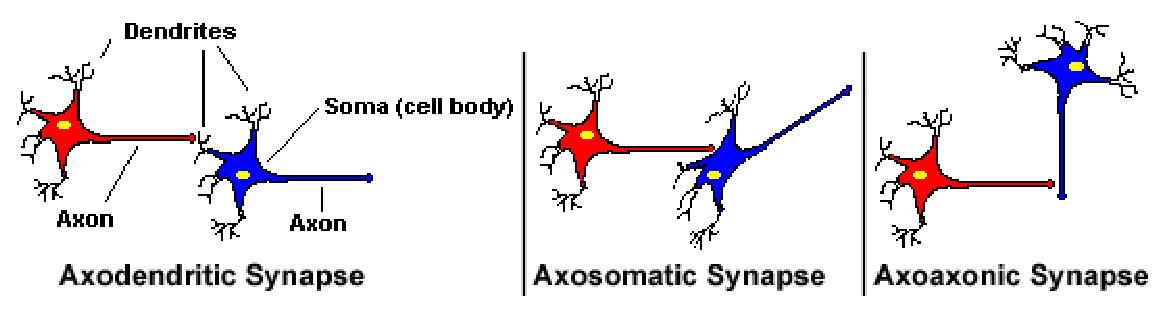
\includegraphics[height=3cm]{./images/synapse_classification_03.eps}}
  \caption{Types of synapses}\label{fig:synapse_classification_03}
%https://faculty.washington.edu/chudler/synapse.html
\end{figure}

\subsection{Neuromuscular junction}
\label{sec:neur-junct}
\label{sec:neuromuscular-junction}

The interface between a motor neuron and muscle fiber is a specialized synapse
called the {\bf neuromuscular junction}. Upon adequate stimulation, the motor
neuron releases a flood of neurotransmitters that bind to postsynaptic receptors
(i.e. Nm type of nAChR - Sect.\ref{sec:nAChR}) and triggers a response in the
muscle fiber. The excitation at the neuromuscular junction is called End-Plate
Potential (EPP) (Sect.\ref{sec:EPP_mechanism}).

% A special type of synapse that forms between axonal terminal of neuron and
% skeletal muscle cell is called {\bf neuromuscular junction} -
% Sect.\ref{sec:neuromuscular-junction}.

\begin{itemize}
\item In invertebrates, depending on the neurotransmitter released and
  the type of receptor it binds, the response in the muscle fiber
  could be either excitatory or inhibitory.

\item For vertebrates, however, the response of a muscle fiber to a
  neurotransmitter can only be excitatory, in other words,
  contractile. Muscle relaxation and inhibition of muscle contraction
  in vertebrates is obtained only by inhibition of the motor neuron
  itself. Although muscle innervation may eventually play a role in
  the maturation of motor activity. This is why muscle relaxants work
  by acting on the motoneurons that innervate muscles (by decreasing
  their electrophysiological activity) or on cholinergic neuromuscular
  junctions, rather than on the muscles themselves.

\end{itemize}

\subsection{calyx of Held synapse}
\label{sec:synapse-calyx-of-Held}
\label{sec:calyx-of-Held-synapse}

Calyx of Held synapse is a large synapse in the mammalian auditory system that
due to its large size, is widely used to study the synapse's electrophysiology
properties, e.g. synaptic plasticity. The name {\bf Calyx}
because its resemblance to the calyx of a flower.





\section{Chemical synapse types and distribution}
\label{sec:synapse-types}
\label{sec:synapse-distribution}

\subsection{GABAergic synapse}
\label{sec:GABAergic-synapse}

GABAergic synapses are found in synapse between a GABAergic interneuron
(Sect.\ref{sec:GABAergic-neurons}) projecting to another neuron.



\subsection{-- catridge synapse}

Axon terminals in chandelier cells (Sect.\ref{sec:chandelier-cells}) form
distinct arrays called "cartridges".

Cartridges is one of the synapse types which show the most dramatic changes
during normal adolescence, which could potentially be relevant to the adult
onset of psychiatric disease. Furthering this link, in schizophrenia, scientists
have observed changes in their form and functionality, such as 40\% decrease in
the axon terminal density.

\url{https://en.wikipedia.org/wiki/Chandelier_cell}



\section{Synaptogenesis vs. Synaptic pruning}
\label{sec:synaptogenesis}
\label{sec:synapse-formation}

{\bf Synaptogenesis} is the formation of new synapses between neurons in the
CNS. The opposite of this is {\bf synaptic pruning} (or axon pruning)
(Sect.\ref{sec:synaptic-pruning}.

Regardless of the different mechanisms of synaptic pruning, in all cases, the
synapses are formed by a transient axon terminal.


\subsection{synaptic pruning}
\label{sec:synaptic-pruning}
\label{sec:axon-pruning}

Synaptic pruning (axon pruning) is the elimination of synapse that occurs
between early childhood and the onset of puberty in many mammals, including
humans.


There are 2 types of pruning
\begin{itemize}
  \item those happens during early development (adolescene): associated with
  learning. They are called {\bf small-scale axon terminal arbor pruning}
  
  \item those happens during aging. They are called {\bf  large-scale
  stereotyped axon pruning}.
  
Hormones and trophic factors are thought to be the main extrinsic factors
regulating  large-scale stereotyped axon pruning.
  
\end{itemize}
While developmental pruning is experience dependent, the deteriorating
connections that are synonymous with old age are not. 

Pruning is influenced by environmental factors and is widely thought to
represent learning. Pruning is thought to be a process of removing neurons which
may have become damaged or degraded in order to further improve the "networking"
capacity of a particular area of the brain. In addition, it is hypothesized as a
means of continually maintaining more efficient brain function by removing
neurons by their synaptic efficiency.

The three models explaining synaptic pruning are 
\begin{enumerate}
  \item axon degeneration, 
  
  \item axon retraction (from distal to proximal order)
  
  \item axon shedding.
\end{enumerate}

However, the molecular mechanism remains unclear.

\section{Axon terminal}
\label{sec:axon-terminal}


The distal ending of the telodendria (Sect.\ref{sec:telodendria}) are called
axonal terminal (synaptic knobs, boutons, terminal button), as shown in
Fig.\ref{fig:terminal_button}.

\begin{figure}[htb]
\centerline{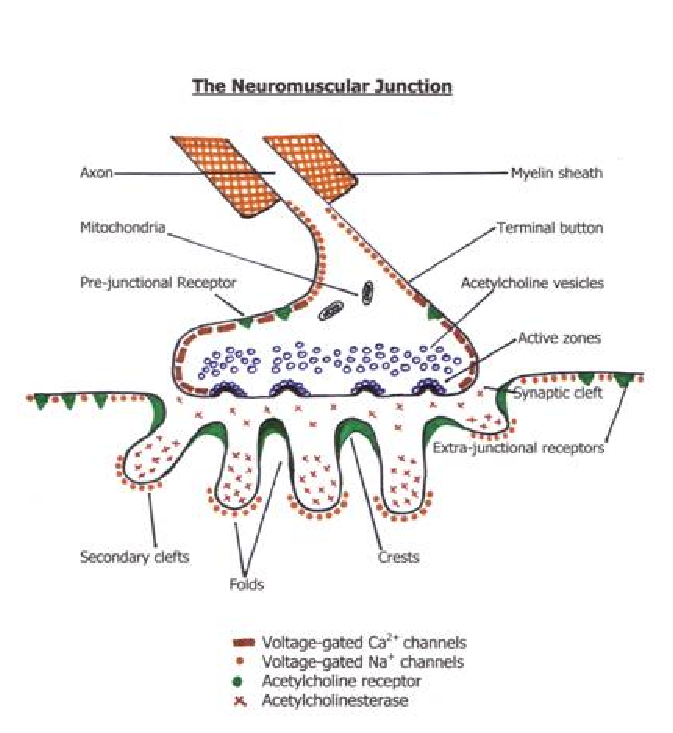
\includegraphics[height=8cm]{./images/terminal_button.eps}}
\caption{Foot-like button of the axon terminal and the junctional
  cleft with a dendrite of a neuromuscular junction}\label{fig:terminal_button}
\end{figure} 

A common observation in studies of neuronal structure is that axons differ in
the size of their synaptic boutons. Yeow - Peterson (1991) used
three-dimensional reconstruction of serial thin sections to examine the
ultrastructure of synaptic boutons that vary in size.
These are synaptic boutons contacting large neurons in the ventromedial gray
matter of the upper cervical spinal cord (probable neck motor neurons).
\begin{itemize}
  \item vary widely: 0.05- 10.1 $\mum^3$
  \item median value: 1.0 $\mum^3$
  \item most boutons are small: 94\% with volume < 4 $\mum^3$; and 74\%with
  volume < 2$\mum^3$; with mean is 1.46$\pm 0.98 \mum^3$
\end{itemize}

The following 4 variables were found to scalewith the bouton size:
1) total active zone area, 2) number of active zones, 3) individual active zone
area, and 4) number of synaptic vesicles. 

Another study using synaptic bouton in the ventral horn in terms of volume,
total surface area and the surface area of apposition to postsynaptic neurons
(apposed surface area), mitochondrial volume, vesicle and active zone features,
relation to presynaptic contacts, postsynaptic profile size, and position within
the terminal arbor.

\begin{table}[hbt]
\small{
\begin{center}
\caption{Axonal terminal}
\begin{tabular}{p{2cm}|p{2cm}p{2cm}p{2cm}p{2cm}p{2cm}} 
  \hline
species/region  & active zone area ($\mum^2$) & bouton size ($\mum^2$) & bouton
volume ($\mum^3$) & bouton length ($\mum$) & mean diameter ($\mum$) \\
  \hline\hline
frog cardiac ganglion & 0.04-1 & 1.5-5.0 & \\
turtle spinal cord & 0.02 - 0.87 & 0.1-4.1 & \\
motoneurons (Ia afferent terminal) & & & 0.5-4.0 \\ 
human cerebral cortex & & & & 0.8 \\
\end{tabular}
\end{center}
\label{tab:axonal-terminal}
}
\end{table}

Bouton in human cerebral cortex in control cells has a much larger range of
perimeter sizes (5.3 $\pm$ 0.4); and a wide range of perimeter size(4.1-8.2
$\mum$, n = 8) than neurons in the undercut cortex (2.7 $\pm$ 0.2 $\mum$; range
2.3$\pm$4.5 $\mum$; p < 0.0006) (Salin - Prince (1995)).

All reconstructed boutons made synapses; the smallest of these fully equipped
boutons had a volume of 0.236 $\mum^3$ (or r=0.68$\mum$). 

\subsection{active zone}
\label{sec:active-zone}

Active zones were identified by pre- and post-synaptic membrane thickenings, at
which synaptic vesicles closely apposed to the pre-synaptic membrane.

An axon terminal can have 1 or more active zones; with for most boutons total
active zone area is small.
In Leow - Peterson (1991)'s study, they claimed that 57\% of found boutons have
total active zone area is < 0.2 $\mum^2$; and 74\% has area < 0.3 $\mum^2$.

\begin{verbatim}
total_active_zone_area = -0.014  + 0.17 * (apposition_area)
\end{verbatim}

Most boutons have 1 or 2 active zones. The great majority have only one active
zone, but 20-25\% have two, and a few contacts bear three or
more.


\subsection{vesicle content}
\label{sec:vesicle-content}

The area in the axon that holds groups of vesicles is
an axon terminal or "bouton" (Sect.\ref{sec:axon-terminal}). 

Yeow - Peterson (1991) suggested that large boutons tend to contain greater
numbers of synaptic vesicles (Sect.\ref{sec:synaptic-vesicles}) than do small
boutons. Thus, they may have a greater capacity for transmitter storage and
release. Interestingly, vesicle number scales linearly with apposition area
(scaling factor = 1.02) rather than with bouton volume \citep{yeow1991}.

Also, vesicle density decreases significantly with bouton volume, but does not
change systematically with apposition area. These data suggest that the synaptic
vesicle population of each bouton forms a layer apposed to the presynaptic
density rather than filling the entire bouton; this vesicle layer increases in
area together with the active zone, but its vesicle density remains invariant.

The mean vesicle density within non-microtubule regions was 1400
vesicles/$\mum^3$ (Pierce-Mendell (1993)), and a similar number 1132
vesicles/$\mum^3$ by Yeow-Peterson (1991).

\textcolor{red}{Vesicle release}: 

\begin{itemize}
  \item Up to 130 vesicles can be released per bouton over a ten-minute period
  of stimulation at 0.2 Hz \citep{ikeda2009}
  
  \item Synaptic vesicles are groupped into 3 different pools:
  reserve pool   (non-recycling pool, NRP), recycling pool (RP), and
  readily-release pool (RRP).
  
  \textcolor{red}{The different pools of vesicles may reflect vesicles near to
  (fast vesicles) and far from (slow vesicles) voltage-gated calcium channels},
  Fig.\ref{fig:vesicle-pool}.
  \begin{enumerate}
    \item RRP =  docked to the cell membrane, making these the first group of
    vesicles to be released on stimulation.
    
   At some synapses the RRP can be divided into fast and slow vesicle pools.
   
Bassoon normally minimizes depression by helping to rapidly replenish vesicles
at release sites (Hallermann et al. 2010). Elevation of $\Ca$ also accelerate
the replenish process of RRP.

   
    \item RP =   There are usually hundreds of vesicles associated with each active zone.
  10-20\% of the vesicle constitute the so-called {\bf recycling pool} (RP).
    
    
    \item NRP =   It is difficult to evoke the release of the remaining pool of vesicles, known
  as the nonrecycling pool (NRP).

     Under experimental conditions, this pool is mobilised by intense
    stimulation, and might occur only once the other two pools are exhausted.
        
  \end{enumerate}
  
\begin{figure}[htb]
  \centerline{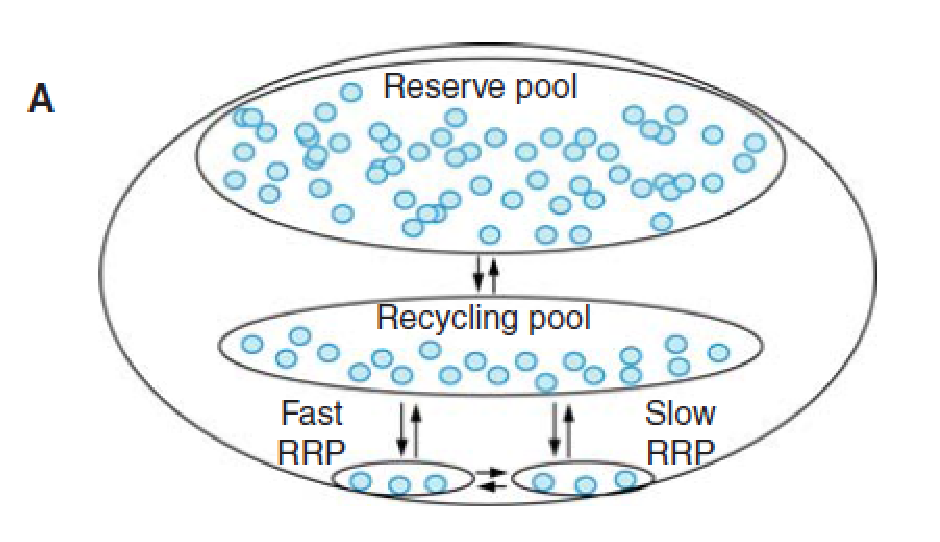
\includegraphics[height=4cm]{./images/vesicle-pool.eps}}
  \caption{Reserve pool, Recycling pool, Fast RRP and
  Slow RRP}\label{fig:vesicle-pool}
\end{figure}

Serial electron microcopy has also been used to determine the number
of morphologically docked vesicles, which may correspond to the RRP.
However, some of the docked vesicles may not be primed, and the RRP need not be
restricted to docked vesicles.
The average number of morphologically docked vesicles at the active zone of
different synapses ranges from two vesicles at the calyx of Held (Satzler et al.
2002) to 27 for inputs onto pyramidal cells in the pyriform cortex (Schikorski
and Stevens 1999).
  
\end{itemize}

\subsection{Vesicle cycle}

\begin{enumerate}
  \item {\bf trafficking to the synapse}: 
  
  \item {\bf transmitter loading}: Once at the synapse, synaptic vesicles are
  loaded with a neurotransmitter (as described above using transport proteins)
  
  \item {\bf docking}: loaded synaptic vesicles must dock near release sites.
  \textcolor{red}{however, the protein play the major role in docking is still
  not known}.
  
  \item {\bf prime}: the process after docking, and before fusion
  
  Priming prepares the synaptic vesicle so that they are able to fuse rapidly in
  response to a calcium influx
  
  \item {\bf fusion}: Primed vesicles fuse very quickly in response to calcium
  elevations in the cytoplasm.
  
  \item {\bf endocytosis}: finally, this process accounts for the re-uptake of
  synaptic vesicles
\end{enumerate}

The release of vesicles out of presynaptic terminal is regulated by a
voltage-dependent calcium channel (Chap.\ref{chap:VDCC_Intro}).





\section{Spine formation}
\label{sec:spine}

Filopodia are thin, actin-rich plasma-membrane protrusions that function as
antennae for cells to probe their environment.
It plays an important role in neurite growth, wound healing, and serves as a
{\it precursor in dendritic spines in neurons}. \citep{mattila2008}

In neuron, as a dendritic spine matures, its morphology changes from a
filopodia-like protrusion to a mushroom-shaped structure. Active Rac1, which is
a small GTPase  that  regulates  actin  dynamics (Sect.\ref{sec:Ras-GTPase}), 
induces the formation of dendritic  spines.
 
Spines continuously change morphology  by  modulating  their  underlying  actin
machinery (Sect.\ref{sec:actin_remodeling}), which has a pivotal role in the
plasticity and integrity of the spine.


\section{Synapses between cells in hippocampal slices}
\label{sec:synaps-betw-cells}

Even though works on cultured cells has provided valuable insights
into mechanism of transmitter action, but neuronal identity and
spatial context may change, e.g. abnormal connectivities may develop
or number of terminals made at a connection may be abnormal high.
Nevertheless, using cultured cells is still the widely used and major
approach to study the electrophysiological properties of cells

There are several pathways in hippocampus
\begin{enumerate}
\item Excitatory postsynaptic potential (EPSP) from granule cell to
  CA3 ({\bf mossy fiber} which are closed to CA3 pyramidal cell soma):
  EPSP of 2-12 mV

\item recurrent EPSP from CA3 pyramidal cell to CA3 pyramidal cell:
  EPSP of 0.6-1.3 mV with the time to peak varies between 5-12 ms. (In
  immature rat, larger recurrent EPSP was observed, i.e. up to 3 mV)

\item EPSP from CA3 pyramidal cell to CA1 pyramidal cell ({\bf
    Schaffer collateral}): EPSP of 0.13 mV in CA1 cells (this low
  amplitude agrees with the observation that spontaneous EPSP are
  difficult to resiolve in CA1 neuron, which is in contrast to large
  EPSP in CA3 cells)

\item EPSP from pyramidal cells to inhibitory cell (in both CA1, CA3):
  EPSP of 2-3 mV

\item Inhibitory postsynaptic potential (IPSP) from CA1 inhibitory
  cell (located in stratum pyramidale) to CA1 pyramidal cell: IPSP of 2-4 mV. It is difficult to
  observe spontaneous IPSP in CA1 cells.

\item IPSP from CA1 inhibitory cells (located in stratu
  lacunosum/moleculare) to CA1 pyramidal cell

\item IPSP from CA3 inhibitory cell (located in stratum pyramidale) to
  CA3 pyramidal cell: these interactions in CA3 cells are more diverse
  than those of the same kind in CA1 cells.

\item Electrotonic interaction between CA3 cells and between dentate cells.
\end{enumerate}


\section{Synaptic vesicles and Neuropeptides}
\label{sec:neurotransmitter-release}

At a single synapse, there can be different types of neurotransmitters, i.e.
co-transmitters. They can be release independent from each other.
In particular, since co-transmitters are often packaged in different types of
vesicles, the transmitters need not be released simultaneously. 
It is believed that the different releases is controlled by different level of
$\Ca$ (Rizzoli, Betz, 2005).

Much of this trigger calcium comes from extracellular fluid and enters the
terminal via Vm-gated $\Ca$ channels during depolarization (Katz, 1969).
$\Ca$ then must be extruded to maintain a steady $\Ca$ balance even when the
neurons fire at rapid rate for long period of time.
\begin{enumerate}
  \item $\Ca$ buffering by cytoplasmic proteins
  
  \item $\Ca$ sequestration/reuptake to ER (via Calmodulin-insensitive,
  ATP-driven SERCA pump) and into mitochondria
  
  \item $\Ca$ extrusion via plasma membrane via Calmodulin-sensitive ATP-driven
  $\Ca$ pump (PMCA) and NCX (Sect.\ref{sec:NCX-isoforms})
\end{enumerate}
NOTE: $\Ca$ buffering and sequestration may be the main mechanism for rapidly
removing $\Ca$ from cytoplasm; and NCX may be the primary mechanism by which
$\Ca$ is extruded from terminals and $\Ca$ balance is restored.
\textcolor{red}{NCX  are present at high concentration in presynaptic
terminals} (Sect.\ref{sec:NCX-distribution}).

At low-frequency stimulus, local elevation of $\Ca$ at axonal terminal mainly
leads to the release of neurotransmitters via synaptic vesicles which holds
small-molecule neurotransmitters in the synaptic cleft
(Sect.\ref{sec:synaptic-vesicles}).

At higher-frequency stimulus, besides the release of synaptic vesicles; the more
available $\Ca$ diffuses to and trigger the release of neuropeptide
(Sect.\ref{sec:neuropeptides}) outside the synaptic cleft.


\url{http://www.ncbi.nlm.nih.gov/books/NBK10818/figure/A383/?report=objectonly}


\subsection{synaptic vesicles}
\label{sec:synaptic-vesicles}

A {\bf synaptic vesicle} in neuron stores various neurotransmitters that are
released at the (chemical) synapse. The term was first introduced by De Robertis
and Bennett in 1954. About 10 years later, they proved that neurotransmitter
acetylcholine is actually contained in synaptic vesicles. Other
neurotransmitters (Sect.\ref{sec:neurotransmitter}) are also found in synaptic
vesicles. The amount of synaptic vesicles available in a presynaptic bouton is
discussed in Sect.\ref{sec:vesicle-content}.

\begin{mdframed}

NOTE: A bacterium has a volume of about 1 $\mum^3$, so the synapse is roughtly
the size of a bacterium.

Rule of thumb: 1 nM concentration in 1 $\mum^3$ is about 1 molecule.
For a vesicle of about $10^{-5} \mum^3$ in volume with 100mM glutamate, there
are about 1000 neurotransmitter molecules in that vesicle. 
  %  nMolecules/(6.022*10^23)/(4/3*3.14*rad^3*1e-24))*1e3 = concentration (mM)
  % rad = radius (nm)
  % 2000 = #molecule/vesicle
  % convert to mole --> devidied by Avogadro number = 6.023*10^23
  %  convert nm^3 to liter --> 1e-24
  %  result is Molar --> convert to mM by multiplying 1e3

\end{mdframed}

In the human brain region V1 synaptic vesicles have an average diameter of 39.5
nanometers with a standard deviation of 5.1 nanometers, i.e. mean spherical
volume $25.8 \times 10^{-5}$.
\footnote{\url{https://en.wikipedia.org/wiki/Synaptic_vesicle}}

  %  (2000/(6.022*10^23)/(4/3*3.14*40^3*1e-24)) * 1e3  = concentration (mM)
  % 2000 = #molecule/vesicle
  % convert to mole --> devidied by Avogadro number = 6.023*10^23
  % spherical volume (nm^3): 4/3*pi*r^3
  %  convert volume (nm^3) to liter --> 1e-24
  %  result is Molar --> convert to mM by multiplying 1e3

Synaptic vesicles contains 2 classes of proteins:
\begin{enumerate}
  \item  transport proteins involved in neurotransmitter uptake:
  It has 

\begin{itemize}
  \item   V-ATPase ($\H$ pumps) to generate electrochemical (proton) gradients
  to allow for neurotransmitter uptake.
  
  \item neurotransmitter transporters that regulate the actual uptake of
  neurotransmitters, i.e.  from the cells' cytoplasm into the synaptic vesicles
  
  These transporters are selective for different classes of transmitters.
  Depending upon the type of neurotransmitters, the amount of protons required
  to uptake one neurotransmitter can change
  \begin{verbatim}
   TYPE                                inward movement          outward movement
norepinephrine, dopamine, histamine, 
serotonin and acetylcholine	           neurotransmitter+	      2 proton
GABA and glycine	                   neurotransmitter	          1 H+
glutamate	                           neurotransmitter- + Cl-	  1 H+  
  \end{verbatim}
\end{itemize}  
  
  \item trafficking proteins (more complex than transport protein) that
  participate in synaptic vesicle exocytosis, endocytosis, and recycling. It has
  \begin{itemize}
    \item intrinsic membrane proteins, 
    
    \item peripherally bound proteins, 
    
    \item proteins such as SNAREs (with more than 60 members) to mediate vesicle
    fusions - that is the fusion of the synaptic vesicle with the target
    membrane bound compartments.
    \url{https://en.wikipedia.org/wiki/SNARE_(protein)}
  \end{itemize}
  
\end{enumerate}

\section{Synapse activation}
\label{sec:synapse-activation}

A brief introduction to synapse is given in Sect.\ref{sec:synapse}.
Upon presynaptic AP, neurotransmitters are release
(Sect.\ref{sec:short-term_potentiation}).

The released neurotransmitter can bind to different possible families of
receptors in the postsynaptic density (PSD) of the dendritic spine
(Sect.\ref{sec:dendritic_spines}).
\begin{itemize}
  \item iGluR - Sect.\ref{sec:iGluR}: ligand-gated ion channels
  \item mGluR - Sect.\ref{sec:mGluR}: G-protein coupled receptors
  \item iGABAR - Sect.\ref{sec:GABA_receptors}: ligand-gated ion channels
  \item mGABAR - Sect.\ref{sec:GABA_receptors}: G-protein coupled receptors
  \item \ldots
\end{itemize}
Each family has many members, and each has its own reversal potential
$E_\rev$.

Each receptor is selectively permeable to particular ions that flow either into
or out of the cell in order to bring the overall membrane potential to this
reversal potential.
\begin{itemize}
  \item if the $E_\rev$ of the bound receptors is higher than the threshold
  potential for the postynaptic neuron, each presynaptic AP triggers an EPSP 
  on postsynaptic side (Sect.\ref{sec:EPSP_mechanism}) and the postsynaptic
  neurons will be more likely to generate an AP.
  
  These synapses are called excitatory synapses.
  
  \item if the $E_\rev$ of the bound receptors is lower than the threshold
  potential for the postynaptic neuron, each presynaptic AP triggers an IPSP
  on postsynaptic side (Sect.\ref{sec:IPSP}) and the postsynaptic neurons will
  be less likely to generate an AP.
  
  These synapses are called inhibitory synapses
\end{itemize}

\subsection{Excitatory Synapse}
\label{sec:excitatory-synapse}

The probability that the single stimulation of an excitatory synapse will raise
the membrane potential past threshold and produce an action potential is not
very high. Therefore, in order to achieve threshold and generate an action
potential, the postsynaptic neuron has the capacity to add up all of the
incoming EPSPs based on the mechanism of summation, which can occur in time and
space.

{\bf Temporal summation} requires high frequency stimulation (tetanic
stimulation) which causes the postsynaptic neuron to sum the incoming EPSPs and
thus increases the chance of the neuron firing an action potential

{\bf Spatial summation} requires activation from multiple synapses. Postsynaptic
neuron can sum together EPSPs from multiple synapses with other neurons.

The neurotransmitters can trigger EPSP
\begin{enumerate}
  \item Acetylcholine (ACh) - Sect.\ref{sec:Acetylcholine}
  
  Found in neuromuscular junctions (control vagus nerve and cardiac muscle
  fiber), skeletal and visceral motor system, and various sites within the CNS. 
  
  \item Glutamate - Sect.\ref{sec:Glutamate}
  
  Found in ???, and bind to NMDAR, AMPAR, and kainate receptors
  (Sect.\ref{sec:glutamatergic_neurons}).
  
  \item Catecholamines - Sect.\ref{sec:Catecholamines}
  
  Epinephrine found in lateral tegmental system, medulla, hypothalamus, and
  thalamus of CNS, and bind to G-protein coupled receptors.
  
  Norepinephrine found in brain stem
  
  Dopamine found mainly in corpus striatum, but also at some other areas in
  brain.
  
  \item Serotonin - Sect.\ref{sec:serotonin}
  
  Found in raphe region of the pons and upper brain stem, extending to the
  forebrain; and bind to 5-HT$_3$ receptors. 
  
  \item Histamine - Sect.\ref{sec:histamine}
  
  There are 4 types of histamine receptors: H1-H4; with H3 is found in CNS.
  
  Found in many regions of brain and spinal cord; and bind to G-protein couple
  receptors.
\end{enumerate}

\subsection{Inhibitory Synapse}
\label{sec:inhibitory-synapse}


The neurotransmitters can trigger IPSP
\begin{enumerate}
  \item GABA - Sect.\ref{sec:GABA}
  
  However, it is important to know that under certain conditions, GABA can still
  be excitatory. {\it In early development phase, GABA, however, have excitatory
  effects}.



  \item glycine - Sect.\ref{sec:Glycine}
\end{enumerate}


\subsection{Electrical behavior of spines}
\label{sec:spines-voltage}


While an excitatory synaptic input may typically generate a $\approx$ 0.5 mV
depolarization at the soma, the magnitude of depolarization at its point of
origin, the dendritic spine, is a subject of debate.
Understanding the electrical behavior of spines has been extremely challenging
because their small size (diameter typically $< 1\mum$) makes them inaccessible
to traditional electrophysiological methods.

\textcolor{red}{Scientific questions}
\begin{enumerate}
  \item What is the peak of $\Vm$ in the spine (i.e. spEPSP) upon synaptic input

  \item Attenuation ratio: spEPSP/soEPSP
  
  The ratio of membrane depolarization in the spine (which is in the range
  10-30mV) to the membrane depolarization in the soma (which is < 1mV).
  
  \item Spine neck resistance: Sect.\ref{sec:spine-neck-resistance}
    
\end{enumerate}

STUDIES:
\begin{enumerate}
  \item {\bf indirect estimate} based on calcium changes measured with
  fluorescent calcium indicators in single spines (Bloodgood et al., 2009;
  Harnett et al., 2012) 

  \item high-resolution stimulated emission depletion imaging, but without
  functional calcium or voltage-imaging (Tonnesen et al., 2014).

  \item voltage sensitive dye (VSD) signals in spines following either
  
  \begin{itemize}
    \item  electrical stimulation of synaptic inputs (Palmer and Stuart, 2009)
    from nearby axons, or
    
    
    
    \item uncaging (Popovic et al., 2015).
    
    the two-photon uncaging approach assures that we can stimulate single
    spines.
  \end{itemize}

  \item single-voxel two-photon VSD imaging to measure backpropagating action
  potentials (bAPs) directly from single spines in acute brain slices (Acker et
  al., 2011; Acker and Loew, 2013). 
  
  \item combine single-voxel two-photon VSD imaging with two-photon
  MNI-glutamate uncaging (Ellis-Davies, 2014) in order to measure the voltage
  responses in individual spines to uncaging-evoked EPSPs (Acker, Loew, 2016).
  
  PROTOCOL: measure the amplitude and dynamics of uncaging evoked EPSPs in
  single spines (called {\bf spEPSP}) on the {\it basal dendrites of L5
  pyramidal neurons} from acute brain slices by uncaging (finer control of what
  spine to be stimulated). At the same time, we measure this uncaging-evoked
  EPSP in the soma with a whole-cell patch and designate this {\bf soEPSP}.

  \textcolor{red}{RESULT}:
  \begin{enumerate}
    \item peak $\Vm$ at spine: spEPSP never exceed 31 mV: with mean peak value
    is 13.0 mV.
    
    soEPSPs are in the range of physiological miniature EPSPs (ie, $< 1$ mV),
    the spEPSP amplitudes never exceed 31 mV (mean 13.0 mV).
    
    \item attenuation ratio: spEPSP/soEPSP $\approx$ 25.3 $\pm$ 12.2
    
  \end{enumerate}
  

\end{enumerate}

\subsection{-- spine neck resistance}
\label{sec:spine-neck-resistance}

The spine neck resistance is a crucial variable that not only controls the
attenuation of synaptic potentials, but also the local amplitudes of synaptic
potentials in spines (Rall, 1974; Gulledge et al., 2012).
 
 \def\Rneck{{\text{R}_{\text{neck}}}}
 \def\MOhm{{\text{M}\Omega}}
 
$\Rneck$
\begin{enumerate}

   \item {\bf hippocampal pyramidal neurons}: 
 
Harnett et al. (2012) - adult rat hippocampal CA1 neuron - tested combining
two-photn calcium imaging, uncaging (glutamate input onto a single spine -
{\bf on apical dendritic trunk}), and pharmacology produced estimates of spine
neck resistances [\textcolor{red}{the postsynaptic EPSP is measured on the
dendritic branch; not on the spine}]: $\approx$ 500 $\MOhm$, with range:
400-600 $\MOhm$. NOTE: This current is purely voltage $\Ca$ channels, as
0.5-1.0 $\muM$ TTX is used (to block sodium channels), 50-100 $\muM$ AP5 is used
(to block NMDAR)

Tonnessen et al. (2014) tested high-resolution stimulated emission depletion
imaging, but without functional calcium or voltage-imaging, estimated spine neck
resistance: $\approx$ 56 $\MOhm$.
  
   \item {\bf cortical pyramidal neurons}:
   
Acker, Loew (2016) - L5 pyramidal neuron within ventral medial prefrontal cortex
(Sect.\ref{sec:ventromedial prefrontal cortex}) tested single-voxel two-photon
VSD imaging (to measure backpropagating action potentials (bAPs) directly from
single spines) combined with two-photon MNI-glutamate uncaging (to measure the
voltage responses in individual spines to uncaging-evoked EPSPs.) estimated
spine neck resistance: 179$\pm$ 25 $\MOhm$. In another 34 spines, using FRAP
(Sect.\ref{sec:FRAP}) cytosolic dyes, together with a novel image processing
method to calculate the spine head volume, the estimated spine neck resistance
for this set of spines are 204$\pm$ 21 $\MOhm$ (not statistically different from
the above method).
   
\end{enumerate}


\subsection{Chemical behavior of spines}

Previous studies have shown the important role that spines can play in the
compartmentalization of synaptic biochemical signals, such as small GTPases and
calcium (Yuste et al., 2000; Murakoshi et al., 2011).



\section{Neurotransmitter}
\label{sec:neurotransmitter}

Neurontransmitters are molecules that neurons released to communicate with
others. NOTE: There is another family of molecules, called neuropeptides -
Sect.\ref{sec:neuropeptides} that neurons also used for communication.

There are about 10 small-molecule neurotransmitters are known
\begin{itemize}
\item ACh : acetylcholine
\item Monoamines:
\begin{itemize}
\item NE
\item DA
\item 5-HT
\end{itemize}
\item Amino acids:
\item Purines: Adenosines, ATP, GTP
\end{itemize}

Depending on the types of neurotransmitters released and the receptor proteins
to which they bind, the result may be either excitation or inhibition of the
postsynaptic neuron. {\bf Acetylcholine} was the first neurotransmitter to be
discovered (in 1921) - Sect.\ref{sec:Acetylcholine}, so the acetylcholine
receptors' kinetics have been intensively studied
(Sect.\ref{sec:acetylcholine_receptor}.

\textcolor{red}{\bf CLASSIFICATION 1}:
\begin{itemize}
  \item inhibitory neurotransmitters: Serotonin (Sect.\ref{sec:serotonin}), GABA
  (Sect.\ref{sec:GABA})
  
  \item excitatory neurotransmitters: Glutamate (Sect.\ref{sec:Glutamate})
  
  \item both excitatory and inhibitory neurotransmitter: Dopamine
  (Sect.\ref{sec:dopamine})
\end{itemize}

\textcolor{red}{\bf CLASSIFICATION 2}: There are currently more than 50
different neurotransmitters in the CNS, but they can be groupped into 4 basic
categories, Fig.\ref{fig:neurotransmitters}:
\url{http://en.wikipedia.org/wiki/Neurotransmitter}
\begin{enumerate}
  \label{sec:neurotransmitter-amino-acids}
  \item {\bf Amino acids}: glutamate (Sect.\ref{sec:Glutamate}), aspartate,
  D-serine, GABA (Sect.\ref{sec:GABA}), glycine (Sect.\ref{sec:Glycine})
  
  \label{sec:neurotransmitter-monoamines}
  \item {\bf Monoamines}: dopamine (DA), norepinephrine (NE, NA noradrenaline),
  epiphrine (adrenaline), histamine, serotonin (SER, 5-HT - Sect.\ref{sec:serotonin}) 
  
  \label{sec:neurotransmitter-peptide}
  \item {\bf Peptides}: somatostatin, substance P, opioid peptides
  (5 members: $\beta$-endorphin, $\alpha$-endorphin, $\gamma$-endorphin,
  $\alpha$-neoendorphin, $\beta$-neoendorphin)  \ldots

Over 50 neuroactive peptides have been found, and new ones are discovered
regularly.
  
  \item OTHERS: Acetylcholine (ACh - Sect.\ref{sec:Acetylcholine}), adenosine, anandamide
\end{enumerate}
NOTE: There are {\bf gasotransmitters} but found in the gastrointestinal: nitric
oxide (NO), carbon monoxide (CO), hydrogen sulfide (\ce{H2S})
\citep{kasparek2008}.   

\begin{figure}[hbt]
  \centerline{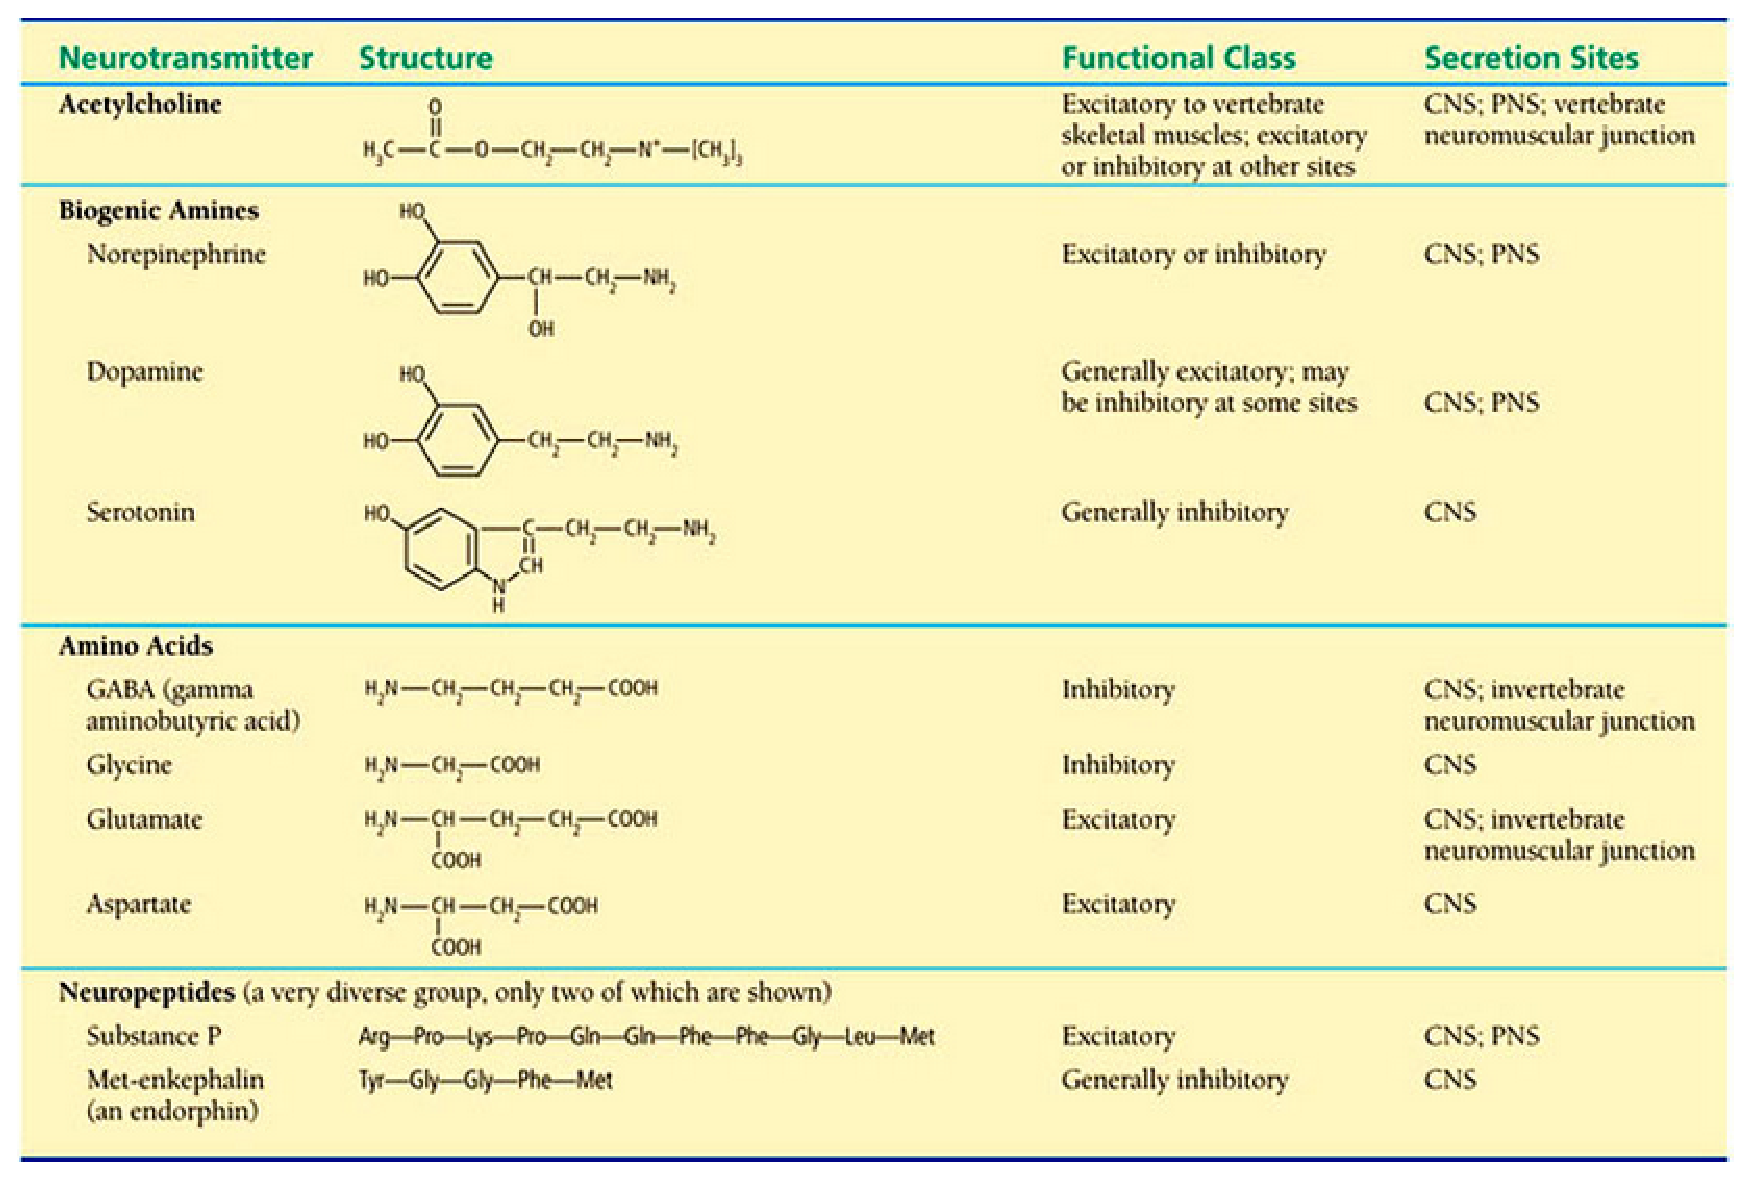
\includegraphics[height=6cm,
    angle=0]{./images/neurotransmitters.eps}}
  \caption{Major neurotransmitters}
  %http://www.apsubiology.org/anatomy/2010/2010_Exam_Reviews/Exam_3_Review/CH_11_Histology_of_the_Neurons_Axon.htm
  \label{fig:neurotransmitters}
\end{figure}


These neurotransmitters function by influencing the trans-membrane ion flow
either as either inhibitory or excitatory.
\begin{itemize}
  \item excitatory: increase the probability that a cell the neurotransmitters
  come in contact will produce an AP
  
  \item inhibitory: decrease  the probability that a cell the neurotransmitters
  come in contact will produce an AP
\end{itemize}
\url{http://en.wikipedia.org/wiki/Neurotransmitter}

The neurotransmitters bind and trigger opening receptor-gated ion channels in
post-synaptic membrane. The opening of these channels enables the positive
charges from outside to enter the neurons, i.e. causing a small localized change
in potential in the post-synaptic membrane of the target neuron - either EPSP or
IPSP (Sect.\ref{sec:postsynaptic_potential}). Multiple events at the same
synapse (temporal summation) or from different synapse on the same neuron
(spatial summation) or both can initiate an electrical change in the membrane of
the dendrite of the neuron leading to a nerve impulse in that cell.

% NOTE: An important concept that aims to explain the mechanism of learning
% and memory is synaptic plasticity (Sect.\ref{sec:synaptic_plasticity}).

The neurotransmitter {\bf acetylcholine} (Sect.\ref{sec:Acetylcholine}), along
with glutamate (Sect.\ref{sec:Glutamate}), is one of the primary excitatory
neurotransmitters in the central nervous system of invertebrates.
GABA (Sect.\ref{sec:GABA}) is the most common inhibitory neurotransmitter
associated with IPSPs in the brain.


\subsection{** Acetylcholine (ACh)}
\label{sec:Acetylcholine}


Acetylcholine (ACh) is the first neurotransmitter to be identified in 1914 by
Henry Dale, for its actions on {\it heart tissue} \cite{Dhir1994PNT}. Its major
function is to activate muscle. This can be done as follows. At the
neuromuscular junction ({\bf end-plate}), the neurotransmitters are released.
When it binds to the receptors on skeletal muscles fibers, it opens {\bf
ligand-gated ion channels} (LGIC or ionotropic receptors) and inducing
contraction of skeletal muscle. However, this is opposite in cardiac muscle
fibers, i.e. it induces decrease contraction. This distinction is attributed to
differences in receptor structure between skeletal and cardiac fibres.
{\it Here the ligands are the neurotransmitters and the receptors are
  LGICs.}


{\bf NOTE:} Besides LGICs, there are also {\bf voltage-gated ion channels}
(open/close dues to changes in membrane potential) and {\bf  stretch-activated
ion channels} (open/close due to the mechanical deformation in the cells).

ACh is synthesized in certain neurons by the enzyme choline acetyltransferase
(the compound of choline and acetyl-CoA).
ACh is synthesized in the cytoplasm of the cholinergic neurons
(Sect.\ref{sec:cholinergic_neurons}.
from choline and acetyl-CoA (Sect.\ref{sec:Acetyl-CoA}). The postsynaptic
receptor for ACh is called acetylcholine receptor
(Sect.\ref{sec:acetylcholine_receptor}).

Each terminal lies on a groove of the muscle fibre junctional cleft, forming a
neuromuscular junction 80\% of acetylcholine is in the vesicle, 20\% in the
axoplasm. About 1/2 million of vesicles in the foot-shaped terminal. Each
acetylcholine vesicle contains approximately 5000 acetylcholine molecules.

\begin{itemize}
\item The precursors is {\bf Choline}
\item The receptors is {\bf nicotinic}, {\bf muscarinic}
\item Synthesizing enzyme is choline acetyltransferase.
\item Deactivated enzyme is acetylcholinesterase.
\end{itemize}

Acetylcholine is vital for neuromuscular transmission.
without acetylcholine, nerve impulse apparently unable to cause contraction in
the muscle fibres.

\begin{figure}[htb]
  \centerline{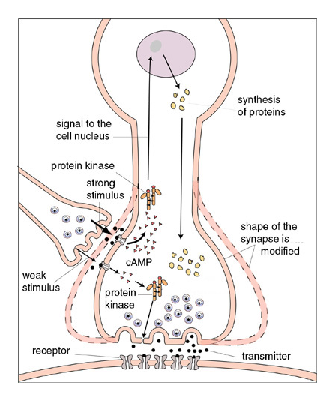
\includegraphics[height=3cm]{./images/synapse-ion_channel.eps}}
  \caption{The synapse with ion channels}\label{fig:synapse_ion-channel}
\end{figure}


\subsection{** GABA (Gamma-AminoButyric Acid)}
\label{sec:GABA}

GABA (Aamma-AminoButyric Acid, $\gamma$-Aminobutyric acid) is the chief
inhibitory neurotransmitter in mammalian CNS (Sect.\ref{chap:CNS}). It is also
found in the GI tract (gastrointestinal).
However, it is important to know that under certain conditions, GABA can still
be excitatory, similar to Glycine (Sect.\ref{sec:Glycine}). 

{\it In early development phase, GABA, however, have excitatory effects}.
In addition, GABA can fulfill many functions, other than simple excitation or
inhibition, such as synchronizing neuronal networks.
It can act as a signalling mediator on the same cell ({\bf autocrine}) as well
as on a different cell ({\bf paracrine}).

GABA synthesis requires Glutamate (Sect.\ref{sec:Glutamate}) using DAG
(Sect.\ref{sec:GAD-enzyme}). GAD uses PLP as a cofactor.
\begin{equation}
\ce{HOOC-CH2-CH2-CH(NH2)-COOH -> CO2 + HOOC-CH2-CH2-CH2NH2}
\end{equation}


GABA are released via vascular transporters
(Sect.\ref{sec:GABA-vesicular-transporter}). Upon release, GABA can binds to
different receptors to trigger the inhibtory effect. These receptors are called
GABA receptors (Sect.\ref{sec:GABA_receptors}).

GABA is a highly flexible molecule; therefore, it can attain many low-energy
conformations that bind to the different GABA receptors.
Two conformationally restricted analogues of GABA are
\begin{enumerate}
  \item extended conformation: E-4- Aminobut-2-enoic acid (trans-4-aminocrotonic
  acid (TACA))

  \item folded conformation: CACA
\end{enumerate}



\subsection{** Glutamate}
\label{sec:Glutamate}

The Glutamate (glutamic acid) is one of 20 amino acids and is best known as
``monosodium glutamate" (MSG) which is used as a flavor or taste enhancer in food. 

Glutamate is the major excitatory neurotransmitter
(Sect.\ref{sec:neurotransmitter}) in the brain.
However, both too much or too low of glutamate is harmful to the brain.
The brain has abundant of glutamate, as much as 5 - 15 mmol glutamate per kg,
depending on the region, more than of any other amino acid; but its role as a
neurotransmitter has not been confirmed until early 1960s and was first found in
insect studies.  Glutamate is also used to synthesize GABA (Sect.\ref{sec:GABA})
- the main inhibitory neurotransmitter of the mammalian CNS.

Almost (99.9\%) of glutamate reside intracellular; but in order to perform as a
neurotransmitter, it needs to bind to the extracellular side of receptors. The
resting concentration of extracellular glutamate is in the range of a few
micromolar ($\muM$); while that inside the cell is several thousand times
higher (1-10 mM). In the nerve terminal and inside synaptic vesicles, the
concentration of glutamate can be as high as 100 mM.

\begin{figure}[htbp]
  \centerline{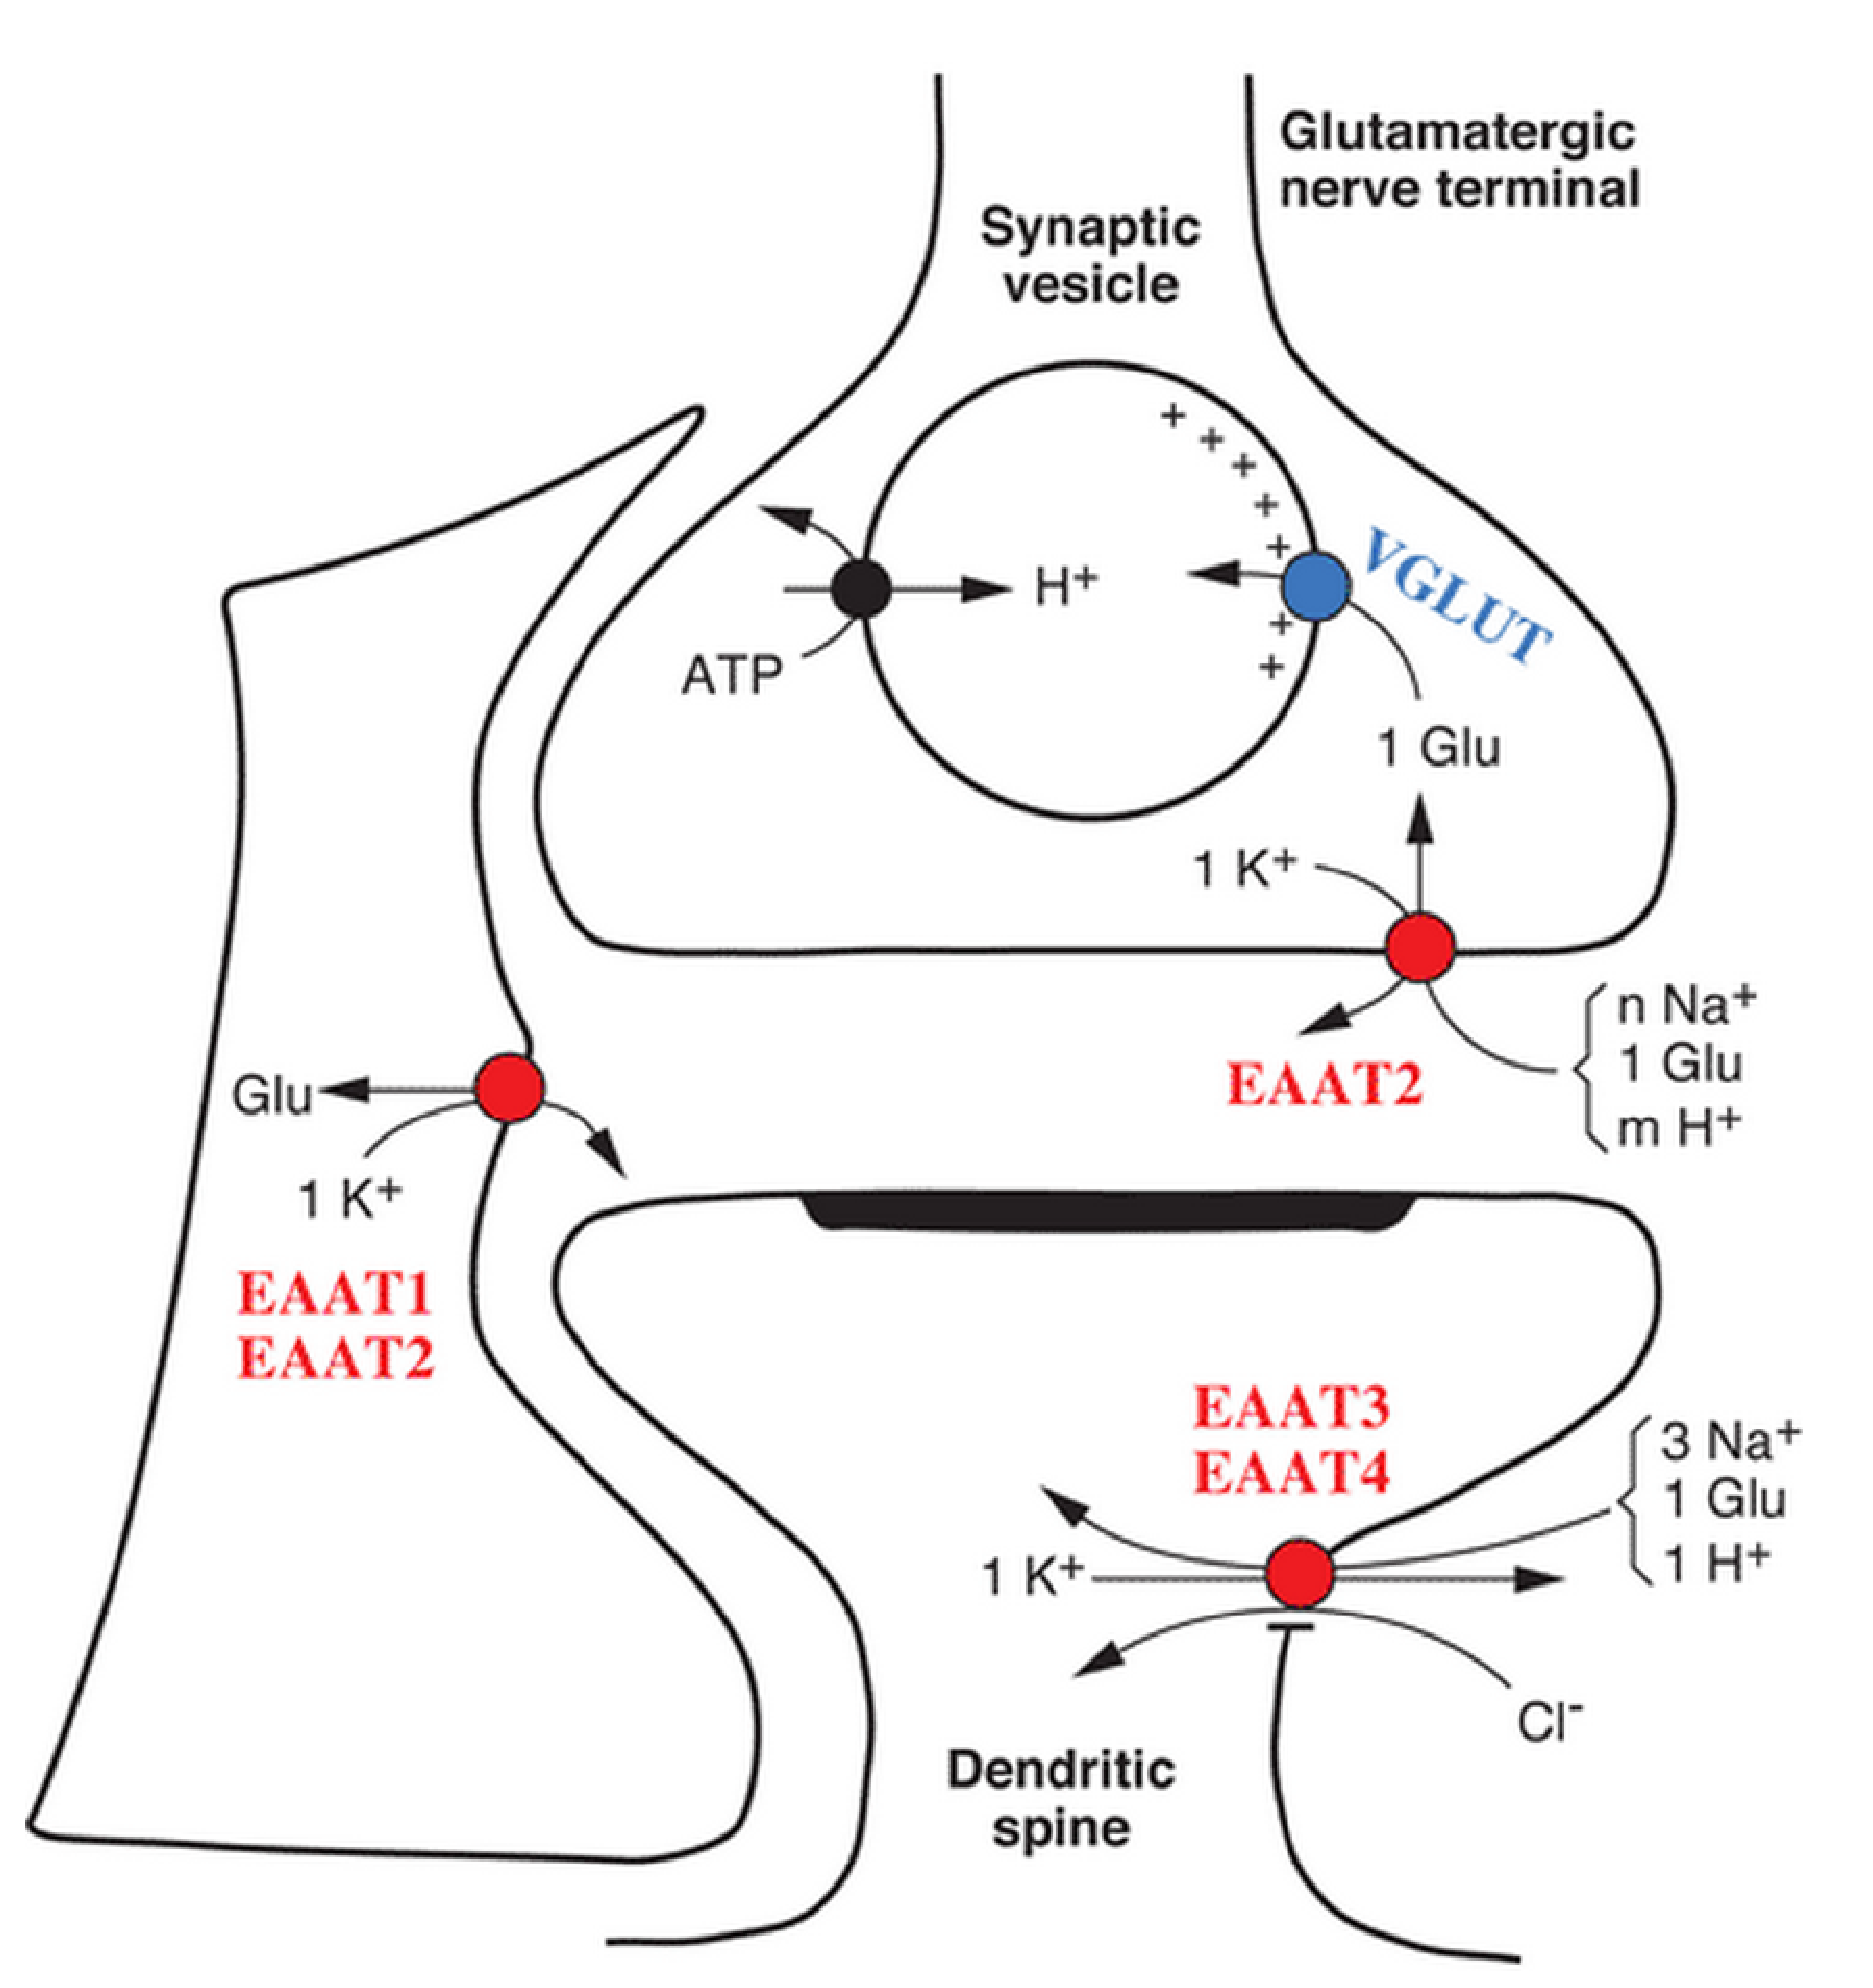
\includegraphics[height=6cm]{./images/Glutamate_uptake.eps}}
  \caption{Glutamate uptake (NOTE: Excitatory Amino Acid Transporters =
EAATs): left-side = astrocyte,
  upper = presynaptic terminal, lower =
  postsynaptic terminal. EAAT2 transports ($n \Na$, 1 Glu, and $n \H$)
  coming into the cell in exchange for 1 $\K$ going out. EAAT3/EAAT3 transports
  ($3 \Na$, 1 Glu, and $1 \H$) coming into the cell in exchange for 1 $\K$
  going out; creating the net effect of 2 extract positive charges entering the cell.
  However, \textcolor{red}{the transpsort occurs slowly} (14 ions/sec) 
  }\label{fig:Glutamate_uptake}
%http://neurotransporter.org/neurotransporters_box.html
\end{figure}

\begin{mdframed}

During normal conditions, \textcolor{red}{glutamate concentration can be
increased up to 1mM in the synaptic cleft}, which is rapidly decreased in the
lapse of milliseconds. When the glutamate concentration around the synaptic
cleft cannot be decreased or reaches higher levels, the neuron kills itself by a
process called apoptosis - Sect.\ref{sec:apoptosis}.

\end{mdframed}


The release glutamate bind to different types of glutamate receptors
(Sect.\ref{sec:glutamate_receptor}), and then extracellular glutamate are
quickly removed by glutamate transporters - Excitatory amino acid transporters
(EAATs), thereby terminating the synaptic transmission
(Sect.\ref{sec:glutamate-glutamine-cycle}).

\subsection{-- Glutamate-glutamine cycle}
\label{sec:glutamate-glutamine-cycle}
%\section{Glutamate-glutamine cycle (GABA)}

Once glutamate released from the axonal nerve terminal, they diffuse to the
postsynaptic side to bind to different receptors to trigger the excitatory
effect. These receptors are called glutamate receptors
(Sect.\ref{sec:glutamate_receptor}).

The concentration of glutamate (Sect.\ref{sec:Glutamate}) in the synaptic cleft
is tightly controlled via the glutamate-glutamine cycle.

\begin{enumerate}

  \item Step 1:
  
Glutamate (mostly L-Glutamate) is taken up into {\bf astrocytes}
(Sect.\ref{sec:glial-cells} by EAAT1/2 (Sect.\ref{sec:EAAT}) which is a
$\Na$-dependent process.

Inside astrocytes, glutamate is converted to the inactive molecule called {\it
glutamine} which is inactive in the sense that it cannot activate glutamate
receptors. This is known as glutamate-glutamine cycle.

EAAT2 glutamate transporter, accounts for >90\% of hippocampal glutamate
re-uptake.

  \item Step 2:

{\it Glutamine}  is then released from the glial cells into to extracellular
fluid to be sequestered back into the {\bf pre-synaptic nerve terminals} (which
can only taken up glutamine, from that it then converts glutamine back to
glutamate for further release) by VGLUT (Sect.\ref{sec:VGLUT}).
\end{enumerate}
 


\url{http://www.abcam.com/neuroscience/glutamatergic-neuron-markers-and-their-functions}




\subsection{Glycine}
\label{sec:Glycine}

Although glycine is structurally the simplest amino acid, it fulfils several
different functions in living organs.
Apart from its role in protein synthesis and metabolism, glycine is a
well-established inhibitory neurotransmitter in the mature nervous system,
especially in the spinal cord and brainstem where it is implicated in the
coordination of reflex responses, in the processing of sensory signals and in
the sensation of pain.

Glycine is released after depolarization from synaptic vesicles contained in the
terminal of interneurons by $\Ca$-dependent exocytosis.
This released glycine can bind to specific receptors (GlyRs) located in patches
in the postsynaptic elements apposed to these terminals, an association that is
inhibited by strychnine.

Glycine molecules and receptors work much in the same way as GABA
(Sect.\ref{sec:GABA}) in the spinal cord, brain (specially the caudal areas),
and retina, i.e. an inhibitory neurotransmitter.
However, Glycine also acts as excitatory in NMDA receptors (Sect.\ref{sec:NMDA})
where glycine is a required co-agonist along with glutamate for NMDA receptors
(Johnson and Ascher, 1987).
\begin{itemize}
  \item Binding of Gly as inhibitory neurotransmitter causes hyperpolarization
  in postsynaptic potential due to influx of $\Cl$ through GlyR
  
  \item Binding of Gly as co-agonist to NMDAR enable NMDAR opening and depolarize postsynaptic potential
  
Early data suggesting that the binding is always, due to (1) high affinity of
glycine site on NMDAR (in low $\muM$ range) and (2) glycine concentration in
synaptic cleft is tonically saturated.

Recent evidences showed that glutamatergic terminal do not contain vesicular
transporter for glycine.
\end{itemize}


\begin{enumerate}
  \item Glycine transporter - Sect.\ref{sec:glycine-transporter} from adjacent
  neuronal and glial process control the concentration of
  Glycine by removing it from glycinergic synapses.
  
  \item Glycine receptor (GlyR) - Sect.\ref{sec:Glycine-receptor},
  Fig.\ref{fig:GABA_receptor}(B).

When glycine receptors are activated, chloride enters the neuron via ionotropic
receptors, causing an Inhibitory postsynaptic potential (IPSP) -
Sect.\ref{sec:IPSP}.

  \item NMDAR - Sect.\ref{sec:NMDAR}
\end{enumerate}

To start a new cycle of release, synaptic vesicles in the nerve terminals have
to be reloaded with glycine from the cytoplasm of the neuron and this occurs
through the action of an intracellular glycine transporter, VIAAT/VGAT
(Sect.\ref{sec:VIAAT/VGAT})


\subsection{Serotonin (SER, 5-HT)}
\label{sec:serotonin}

{\bf 5-hydroxytryptamine (5-HT)} (Serotonin, SER) was first discovered in 1940s,
and within a decade after, they were confirmed as a neurotransmitter.

% About 90\% of the human body's serotonin  located in the enterochromaffin cells
% in the GI tract, where it is used to regulate intestinal movements.
% The remainder is synthesized in serotonergic neurons of the CNS, where it has
% various functions.

5-HT is found mainly in  gastrointestinal tract (GI tract), with 90\% of human
body 5-HT is in  enterochromaffin cells of the GI tract, 
and then in raphe nucleus of the CNS (Sect.\ref{sec:raphe-nuclei}), blood
platelets.

\begin{enumerate}

  \item  From GI tract, after finding its way into the blood, 5-HT are actively
  taken up by blood platelets which store them so that when the blood platelets
  bind to a clot, they release serotonin to regulate the blood clotting.

  \item The reamining serotonin is synthesized by serotonergic neurons
(Sect.\ref{sec:serotonergic-neuron}) found in raphe nuclei
(Sect.\ref{sec:brain-stem}), and upon releases, they bind to 5-HT
receptors (Sect.\ref{sec:5-HT_receptor}).

Serotonin is released as neurotransmitter but also released non-synoptically
through some axon terminals. Serotonergic neurons projects to almost everywhere in the brian
(Sect.\ref{sec:raphe-nuclei}).
\end{enumerate}

{\bf SYNTHESIS}: 
\begin{verbatim}
5-HTP --[DOPA decarboxylase]-->   5-HT
        [and PLP]
\end{verbatim}

PLP = pyridoxal phosphate (the active form of vitamin B6) as cofactor in the
reaction.


\subsection{** Catecholamines: Dopamine, Norepinephrine, Epinephrine}
\label{sec:Catecholamines}

% Three main types of catecholamines in human body are dopamine, norepinephrine NE
% (used to be called noreadrenalin) or epinephrine (used to be called adrenalin).

Catecholamine refers to a class of monoamine derived from tyrosine amino acid
(Sect.\ref{sec:amino-acid}).

\begin{verbatim}
phenylalanine --[hydroxylation via enzyme ]---> L-tyrosine
                [phenylalanine hydroxylase]
                [with copper as co-factor]
dietary protein ----> L-tyrosine           

L-tyrosine -[tyrosine hydrolase]--> L-DOPA --[via DOPA decarboxylase]--> dopamine [and PLP]

dopamine ---[on some cell types]---> norepinephrine --> epinephrine
    norepinephrine --[(PNMT)]->   epinephrine
    
    PNMT = phenylethanolamine N-methyltransferase enzyme 
\end{verbatim}
NOTE: dopa (dihydroxyphenylalanine); PLP = pyridoxal phosphate (the active form
of vitamin B6) as cofactor in the reaction.

Tyrosine hydrolase is a rate-limiting enzyme that involves in DOPA biosynthesis.
It uses tetrahydrobiopterin and molecular oxygen to convert tyrosine to
DOPA.
% and phenylalanine, any of various naturally occurring amines that function as
% {\it neurotransmitters} and {\it hormones} within the body.

There are 3 main catecholamines in human body: 
\begin{enumerate}
  \item dopamine - Sect.\ref{sec:dopamine} 
  
  \item norepinephrine (used to be called noreadrenalin) - Sect.\ref{sec:norepinephrine}

  \item epinephrine (used to  be called adrenalin) - Sect.\ref{sec:epinephrine}
\end{enumerate}
% All of which are produced from phenylalanine and L-tyrosine, according to the
% following sequence
% \begin{verbatim}
% tyrosine ---> dopa (dihydroxyphenylalanine) ---> dopamine 
%    ---> norepinephrine (noradrenaline) ---> epinephrine (adrenaline)
% \end{verbatim}

Depending upon the type of catecholamines and the location where catecholamines
are synthesized, it can play different roles: synthesized in the brain
(functioning as a neurotransmitter), in the adrenal medulla of the adrenal gland
in the kidney (functioning as a hormone - Sect.\ref{sec:adrenal-gland}), and by
some sympathetic nerve fibres (functioning as a neurotransmitter).

\begin{itemize}
  
  \item norepinephrine (Sect.\ref{sec:norepinephrine}) and dopamine
  (Sect.\ref{sec:dopamine}), act as neurotransmitters in the central nervous
  system and as hormones in the blood circulation.

  \begin{enumerate}
    \item  nerve cell: The particular catecholamine that is synthesized by a nerve
    cell, or neuron, depends on which enzymes are present in that cell. 
    
    \item One typical effect of these hormone is to increase the heart rate,
    i.e. fight-or-flight response (Sect.\ref{sec:heart-rate}).
    Catecholamines have a half-life of a few minutes when circulating in the blood.
    
  \end{enumerate}  
  
  \item  norepinephrine is a neurotransmitters of the peripheral sympathetic
  nervous system.
\end{itemize}
\url{http://www.britannica.com/EBchecked/topic/99345/catecholamine}

Upon released, catecholamines act exclusively on adrenergic receptor (AR) -
Sect.\ref{sec:adrenergic_receptor}, which is a type of G protein couppled
receptor, with complex effects.
% Thus, we also need to understand GPCR well enough
\begin{enumerate}
  
  \item Dopamine (Sect.\ref{sec:dopamine}): elicits hyperactivity and repetitive,
  stereotyped behavior activation of dopamine receptors on medulla: inhibit
  vomitting; so antagonist to these receptors can induce vomitting to patients
  after poisoning or drug overdose.

  

  \item Norepinephrine (NE, Sect.\ref{sec:norepinephrine}): acts on $\alpha$-AR
  (both 1 and 2), and only $\beta_1$-AR only.
  
  \item Epiphrine (Sect.\ref{sec:epinephrine}): acts on $\alpha$-AR (both 1 and
  2), $\beta_1$-AR and $\beta_2$-AR.
\end{enumerate}

\subsection{-- Dopamine (DA) 3,4-dihydroxyphenylethylamine}
\label{sec:dopamine}

{\bf Dopamine} (DA, 3,4-dihydroxyphenylethylamine) is one type of catecholamines
(Sect.\ref{sec:Catecholamines}). The catalytic of DA starts with tyrosine
hydrolase (Sect.\ref{sec:tyrosine-hydroxylase}).
\begin{verbatim}

tyrosine --[tyrosine hydrolase]--> L-DOPA -->...--> DA
\end{verbatim}
Tyrosine hydroxylase is the rate limiting enzyme in this pathway, also referred
to as the catecholamine synthesis pathway.  

The product from further metabolic modification of dopamine is Epinephrine and
Norepinephrine (Sect.\ref{sec:epinephrine}).


DA is largely produced in neuronal cell bodies of dopaminergic neurons
(Sect.\ref{sec:dopaminegic_neurons}), and in adrenal medulla
(Sect.\ref{sec:adrenal-medulla}).
Upon released from dopaminergic neurons, DA binds to dopamine receptors on the
postsynaptic side of the projected neurons (Sect.\ref{sec:dopamine_receptors}).
DA and related compounds may exert their effects not only at receptors for DA,
but also at adrenoceptors (Sect.\ref{sec:adrenergic_receptor}).

In the central nervous system (CNS), dopamine is involved in the control of
locomotion, cognition, affect and neuroendocrine secretion. The dysregulation of
dopamine release and neurotransmission are involved, directly or indirectly, in
several brain dysfunction and pathophysiology of many diseases, such as
Alzheimer's disease, schizophrenia, Parkinson's disease, attention deficit
hyperactivity disorder, depression and drug addiction, leading to the clinical
use of drugs that target dopamine neurotransmission in the treatment of these
disorders.
\begin{enumerate}
  \item degeneration of dopamine neurons in the substantia nigra contributes to
  the pathogenesis of Parkinson's disease (Sect.\ref{sec:Parkinson-disease}.
  
  
  \item Schizophrenia (Sect.\ref{sec:schizophrenia})
\end{enumerate}

As DA receptors (Sect.\ref{sec:dopamine_receptors}) are the primary targets of
drug action, it has been suggested that : (1) substitute with dopamine receptor
agonist (function like dopamine), (2) increase dopamine precursor L-DOPA (help
to compensate for the lac of endogenous dopamine production)


\subsection{----- DA release}

DA release is controlled by
\begin{enumerate}
  \item stimulation-dependent DA release
  
  \item D2-like dopamine autoreceptors (Sect.\ref{sec:dopamine_receptors}) on
  presynaptic side that upon activation, inhibit stimulation-dependent DA release
  
  \item 
\end{enumerate}

\subsection{----- DA sensing}
\label{sec:dopamine-theurapeutic-role}

Dopamine transduces its various effects depending upon the type of dopamine
receptors - Sect.\ref{sec:dopamine_receptors}.

\textcolor{red}{\bf In heart}:
\begin{itemize}
  \item At low concentrations (though still enough to activate D1R), the primary
cardiovascular effect of DA is on the vascular D1-receptors. 

  \item At somewhat higher concentrations, DA exerts a positive inotropic effect
  on the myocardium by acting not only at DA receptors, but on $\beta$1-adrenergic
receptors (Sect/\ref{sec:beta-1-adrenergic-receptor}).

  \item At high concentrations, DA stimulates $\alpha$1-adrenergic receptors,
  leading to vasoconstriction (Sect.\ref{sec:alpha-1-adrenergic-receptor})
\end{itemize}
Due to the complex effect, the use of DA in the treatment of life-threatening
states of shock requires careful hemodynamic monitoring.





\subsection{----- DA concentration}

\textcolor{red}{\bf DA measurement}:
\begin{itemize}
  \item fast-scan cyclic voltammetry (FSCV) - Sect.\ref{sec:FSCV}:
  sensitive down to 1 nM 
\begin{verbatim}
Tonic:
  - 5-20 nM based on microdialysis or differential non-pulse voltammetry
  - 50-100 nM based on theoretical estimation of FSCV and pharmacologic studies

Phasic: extracellular dopamine is known to reach high concentrations for brief
   periods (most likely as a result of concerted bursting firing of DA neurons
   often occur on presentation of salient sensory input)   

  - peak > 1 uM , high enough to activate low-affinity D1- and D2-receptors

\end{verbatim}
  
  
\end{itemize}
% In the brain, dopamine (Sect.\ref{sec:dopamine}) is produced by
% dopaminegic neurons (Sect.\ref{sec:dopaminegic_neurons}).





\subsection{----- DA downstream effect signaling pathways}
\label{sec:dopamine-signaling-pathway}

Dopaminergic pathways has been implicated in several major neurologic and
psychiatric disorders.

Depending on the receptors that DA binds to, it may creates opposite downstream
effect. The center of these signaling pathway is DARPP-32 which is expressed in
medium-sized spiny neurons.

\begin{enumerate}
  \item DA -> D1R opening -> enhance cAMP level -> phosphorylated DARPP-32 at
  Thr34:
  
  \item DA -> D2R opening -> reduce cAMP level
\end{enumerate}




\subsection{-- Epinephrine, Norepinephrine (noreadrenalin)}
\label{sec:norepinephrine}
\label{sec:epinephrine}
\label{sec:noradrenalin}

\begin{mdframed}

Oral dosing of norepinephrine or epinephrine is not possible due to the rapid
metabolism of catechol nucleus in gastrointestinal mucosa and liver. Therefore,
these agents are given via I.V., I.M., topically and in aerosol sprays.

Epinephrine is often used in combination local anesthetic agents to prolong the
duration of anesthetic action, i.e.
epinephrine can induce vasoconstriction thus limiting the diffusion of the local
anesthetic from the site of injection. The anesthetic agent would include
articaine, bupivacaine or lidocaine.
This not only prolongs the actions of the local anesthetic but also to reduce
the toxicity of the local anesthetic by limiting its systemic absorption.
Lidocaine in toxic doses can produce cardiac arrthythmias and convulsions.
\url{http://www.uky.edu/~mtp/OBI836AR.html}
\end{mdframed}

Epinephrine and Norepinephrine is the product from further metabolic
modification from dopamine (Sect.\ref{sec:dopamine}) in some cell types.
\begin{verbatim}
dopamine --[DBH       ]--> norepinephrine
           [and Oxygen]
           
norepinephrine --[PNMT                       ]--> epinephrine
                [and  S-adenosyl-L-methionine]
\end{verbatim}
enzyme dopamine $\beta$-hydroxylase (DBH) use $\ce{O2}$ as co-factor, 
and enzyme phenylethanolamine N-methyltransferase (PNMT) uses
S-adenosyl-L-methionine as co-factor. 

Recent evidences have showed that noradrenalin can be released by lactate
(Sect.\ref{sec:lactate}) from noradrenergic neurons
(Sect.\ref{sec:noradrenergic-neurons}) - Tang et al.
(2014).

\subsection{----- Norepinephrine (NE)}

{\bf Noradrenergic system} refers to the involving norepinephrine in the
transmission of nerve impulses.
Norepinephrine (NE) is released in the neocortex after activation of the {\it
locus coeruleus} of the brain stem in response to a number of behavioral
conditions, e.g. stress, novel, salient, fear (fight-or-flight stimuli) or
sexual activities; and the {\it lateral tegmented field}. The neurons in these
areas project to multiple brain areas including the amygdala, spinal cord,
hippocampus, thalamus, hypothalamus, and importantly, the neocortex
(review: \citep{dinh2009}).

With a prominent projections from the {\bf locus coeruleus} of the brainstem to
the temporal region of the neocortex (especially the {\bf prefrontal cortex} and
motor cortex), a large body of results has implicated the role of brain stem
noradrenergic system in learning, attention, and integrative functions in the
neocortex; yet with different reported results (Berridge et al. 1993; Berridge
and Waterhouse 2003; Arnsten and Li 2005; Ramos and Arnsten 2007) (review:
\citep{salgado2009}).


\textcolor{red}{Norepinephrine (NE)}: acts on $\alpha$-AR (both 1 and 2), and
only $\beta_1$-AR only (Sect.\ref{sec:adrenergic_receptor}); which alters both
cortical glutamatergic as well as $\gamma$-aminobutyric acid (GABA)ergic
synaptic transmission

Effects on glutamatergic system
\begin{itemize}
  \item NE facilitate Glu-evoked excitatory synaptic transmission
 
 The application of NE (1-35 nA; 4-25 min duration) can improve the
 somatosensory cortical neuronal response to iontophoretic pulses of
 acetylcholine (ACh) or glutamate (Glu) (10-60 nA; 5-25 s duration) with 94\%
 (Glu) and 67\% (ACh).
  
 The mechanism: NE activate $\alpha_1$-AR, trigger PKC.
 IMPORTANT: This does not requires $\beta$-AR activation or intracellular
 increase in cAMP \citep{mouradian1991}.
 
  
A puzzling issue is that NE has been associated with both
increases and decreases in cortical excitability
\begin{itemize}
  \item NE depresses AMPAR-dependent and non-NMDAR-dependent 
  EPSCs 
  
  \item NE induces $\alpha_1$-AR mediated increase  
\end{itemize}

\begin{enumerate}
  \item NE induces $\alpha_1$-AR mediated decrease 
  the amplitude of IPSC evoked by stimulation of layer I
  
  \item NE induces $\alpha_2$-AR and $\beta_1$-AR mediated increase
  the amplitude of IPSC evoked by stimulation of layer II/III.
  
\end{enumerate}
\end{itemize}

Effects on glutamatergic system
\begin{itemize}  
  \item NE modulate inhibitory synaptic transmission

NE exerts an overall inhibitory action on baseline neuronal activity (Foote et
al. 1975; Manunta and Edeline 1997, 1998) and induces frequency-selective
changes in the tuning curves (Manunta and Edeline 2004).
  
\end{itemize}
 

\subsection{----- Epiphrine}

\textcolor{red}{Epiphrine}: acts on $\alpha$-AR
(both 1 and 2), $\beta_1$-AR and $\beta_2$-AR.
 
 \subsection{** Endocannabinoid (eCB)}
\label{sec:endocannabinoid}
\label{sec:eCB}


Endogenous cannabinoids (eCB) refer to cannabinoid-like molecule produced by the
body (Sect.\ref{sec:cannabis}). There are two discovered types of eCB

\begin{enumerate}
  \item {\bf Anandamide} (Sect.\ref{sec:anandamine}): 
  
  \item {\bf 2-AG} (Sect.\ref{sec:2-AG}):  
\end{enumerate}
% eCB is released (Sect.\ref{sec:endocannabinoid}) from postsynaptic side and
% then bind to CB1R on presynaptic side (Sect.\ref{sec:CB1R}). 

eCB  are released from depolarized postsynaptic neurons in a $\Ca$-dependent
manner and act retrogradely onto presynaptic cannabinoid receptors (CBR -
Sect.\ref{sec:cannabinoid-receptors}, with CB1R in brain) to suppress the
release of neurotransmitter in both excitatory and inhibitory synapses
(Sect.\ref{sec:retrograde-signaling-pathway}). eCB involve in a variety of
physiological processes including appetite, pain-sensation, mood, and memory.


\subsection{-- 2-AG (2-arachidonoylglycerol)}
\label{sec:2-AG}
\label{sec:2-arachidonoylglycerol}

2-AG is sn-2-arachidonylglycerol (Mechoulam et al., 1995,
Sugiura et al., 1995) is one type of eCB (Sect.\ref{sec:endocannabinoid}).

2-AG is biosynthesized by phospholipase  C$\beta$ (PLC$\beta$ -
Sect.\ref{sec:PLC-beta}) and DAG lipase (Sect.\ref{sec:DAG}), and this
biosynthesis also requires $\Ca$ for catalytic function, though the $[\Ca]$ for
maximum activation is different in different PLC isozymes (Sect.\ref{sec:PLC})

Compared to the other eCB anandamine, 
\begin{enumerate}
  \item   2-AG can reach 170x higher in
concentration that anandamine in the brain (Stella, 1997), even though it was
undetectable in striatum at that time.

  \item 2-AG is a full CB1R agonist; whereas anandamide is a partial agonist
  (Sugiura 1999)
\end{enumerate}

In the hippocampus, 2-AG is relased, but not anandamide, after glutamatergic
input.


Among 5 types of PLC: only PLC$\beta$ are activated by mGluR1
(Sect.\ref{sec:mGluR1}) and M1/M3 muscarinic receptors
(Sect.\ref{sec:M1-muscarinic-receptor}, Sect.\ref{sec:M3-muscarinic-receptor}).
 
\subsection{-- Anandamine (AEA)}
\label{sec:anandamine}

Anandamide was first found as an endogenous cannabinoid in 1992 (Devane et al.,
1992) - Sect.\ref{sec:endocannabinoid}). 

Anandamide is formed through the pathways that involve
\begin{enumerate}
  
  \item trans-acylation of the amino group of phosphatidylathenolamine 
  with arachidonate from sn-1 position of phosphatidylcholine
  
  
  \item   D-type phosphodiesterase activity on the resuslting NAPE
  (N-arachidonylphosphati-dylethanolamide)
  
\end{enumerate}
Synthesis of anandamide is regulated by both enzymes:  N-acyl-transferase and
phospholipase D (Sect.\ref{sec:phospholipase}); by stimuli that raise $[\Ca]_i$
or by receptors that linked with cAMP and PKA. Aandamide is formed when the
neuron is depolarized, i.e. $[\Ca]_i$ is elevated (Cadas, 1996).

\begin{itemize}
  \item After D2R activation (Sect.\ref{sec:D2-like-receptors}, iSPN) :
  anandamide is produced; not 2-AG

Adandamide is suggested to function as a local neuromodulator with negative
feedforward regulatory effect of D2-mediated locomotor behavior (Giuffrida,
1999)

\end{itemize}

Anandamide's long hydrocarbon tail makes it fat-soluble and allows it to easily
slip across the hydrocarbon-rich curtain that isolates the brain from the
bloodstream. Notice that its three-dimensional shape strongly resembles that of
THC (Sect.\ref{sec:THC}).

Drugs with similar or stronger behavior:
\begin{enumerate}
  \item \ldots
\end{enumerate}
The key was isolated by Israeli scientist Raphael Mechoulam in 1992: arachidonyl
ethanolamide, later called 'anandamide'


\subsection{** Enkephalins and Endorphins}
\label{sec:enkephalins}
\label{sec:endorphins}

Enkephalins is pentapeptide, endogenous ligand found in some neurons
(Sect.\ref{sec:enkephalin-containing-neurons}).
There are three well-characterized families of opioid peptides produced by the
body: enkephalins, endorphins, and dynorphins.  They are considered as the
body's natural painkillers (endorphins and enkaphalins).

Drugs with similar or stronger behavior:
\begin{enumerate}
  \item morphine (Sect.\ref{sec:morphine})
\end{enumerate}




\section{Presynaptic side}
\label{sec:presynaptic-side-structure}

\subsection{synaptophysin}
\label{sec:synaptophysin}

Synaptophysin (also known as the major synaptic vesicle protein p38) is the
major integral membrane glycoprotein of neuronal synaptic vesicles present in
virtually all synapses and shows a high degree of evolutionary conservation
across the mammals. The protein, in humans, is encoded by the SYP gene.

\subsection{$\Ca$ channels}

$\Ca$ channel is discussed in Sect.\ref{chap:VDCC_Intro} The members of the
Ca(v)2 calcium channel family are located predominantly at presynaptic nerve
terminals, where they are responsible for controlling evoked neurotransmitter
release.

\subsection{CB1R}

Sect.\ref{sec:CB1R}

\subsection{mGluR}

Sect.\ref{sec:mGluR-presynaptic}

\subsection{+ mGluR}

Sect.\ref{sec:mGluR-presynaptic}

\subsection{+ GABAR-autoreceptor}

Sect.\ref{sec:GABA-receptor-presynaptic}

\subsection{+ A2A receptor}
\label{sec:A2AReceptor-pre-synapse}

To discuss A2A receptor on post-synaptic side, check Sect.\ref{sec:A2AReceptor-post-synaptic-side}

A2A receptor (Sect.\ref{sec:adenosine-receptor})
\begin{enumerate}
  \item in cortical glutamatergic terminal: 
  where A2A receptors heteromerize with A1 receptors (A1Rs) and where they
  perform a fine-tuned modulation of glutamate release (Ciruela et al., 2006;
  Quiroz et al., 2009).
  A1R-A2AR heteromers seem to work as a concentration-dependent switch (Ferre
  et al., 2007), with adenosine acting primarily at A1Rs at low concentrations,
  and at both A1Rs and A2ARs at higher concentrations. 
  
Interestingly, presynaptic A2ARs are preferentially localized in glutamatergic
terminals of cortico-striatal afferents to the dynorphinergic MSN (Quiroz et
al., 2009). 
  
Activation of the A1R in the A1R-A2AR heteromer produces inhibition of glutamate
release, while the additional activation of the A2AR produces the opposite
effect, on a mechanism that seems to involve an allosteric modulation in the
receptor heteromer and interactions at the G protein level (Ciruela et al.,
2006; Ferre et al., 2007).     

 A2ARs are also localized presynaptically, in cortico-striatal glutamatergic
 terminals that contact the striato-nigral MSN (D1+ MSN) These presynaptic A2ARs
 heteromerize with A1 receptors (A1Rs) and their activation facilitates
 glutamate release. \citep{ferre2011}
  
  Adenosine A1 and A2A receptors are co-expressed in pyramidal neurons and
  co-localized in glutamatergic nerve terminals of the rat hippocampus. 
  
  
    \item in hippocampus:

 Hippocampal A(2A) receptors (in rat) are enriched in synapses, mainly in the
 active zone of nerve terminal, in accordance with their role in controlling
 neurotransmitter release \citep{rebola2005}
    
  The binding density of A2A receptor's antagonist [(3)H]SCH 58261 for total
  membranes (B(max)=29+/-4 fmol/mg protein) from the hippocampu; while that in 
  nerve terminals membranes is about 3x higher (B(max)=103+/-12 fmol/mg
  protein).
  
  
\end{enumerate}

\subsection{Alpha-synuclein protein (SCNA gene)}
\label{sec:alpha-synuclein}
\label{sec:SNCA-gene}

{\bf Alpha-synuclein} ($\alpha$-synuclein or $\alpha$Syn) protein is abundant in
the brain (and is found mainly at the tip of nerve cells - presynaptic
terminals) (Stefanis, 2012). Smaller amounts are found in the heart, muscles,
and other tissues.
% https://www.ncbi.nlm.nih.gov/pmc/articles/PMC3281589/


The protein is small, i.e. 140 amino acids (encoded by SCNA gene), making up
about 1\% of proteins in cytosol in neurons of neocortex, hippocampus,
substantia nigra, thalamus, and cerebellum; though it is also found in glial
cells (Sect.\ref{sec:glial-cells}).

\begin{itemize}
  
  \item  In neurons, it is found predominantly in presynaptic termini, in both
  free- and bound- forms (with 15\% of synuclein in membrane-bound form in any
  moments in neurons).
  
  
  The N-terminus of $\alpha$Syn contains seven 11-residue repeats that form an
  amphipathic helix on membrane binding (Davidson et al., 1998; Bussell and
  Eliezer, 2003), and this membrane binding contributes to its presynaptic
  localization (Fortin et al., 2004), i.e.  $\alpha$Syn is a peripheral membrane
  protein that localizes specifically to the axon terminal in neurons,
  suggesting a role in neurotransmitter release (Maroteaux et al., 1988; Iwai et
  al., 1995), though as you will see below, the role is not yet clear.
  

  \item Recent data also suggest alpha-synuclein localized in neuronal
  mitochondria, in particular the inner membrane with its  inhibitory effect of
  alpha-synuclein on complex I activity of mitochondrial respiratory chain is
  dose-dependent.
  
Alpha-synuclein is highly expressed in the mitochondria in olfactory bulb,
hippocampus, striatum and thalamus, where the cytosolic alpha-synuclein is also
rich. However, the cerebral cortex and cerebellum are two exceptions, which
contain rich cytosolic alpha-synuclein but very low levels of mitochondrial
alpha-synuclein


Accumulation of $\alpha$-synuclein into mitochondria can lead to their dysfunction and
$\alpha$-synuclein overexpression has been associated with complex I dysfunction.

The N-terminal domain of $\alpha$-synuclein has been found to be relevant to target the
protein to complex I  and domain integrity is necessary for the control of
neuronal mitochondrial morphology

A fraction of soluble $\alpha$-synuclein is targeted to mitochondria and appears to
interact directly with mitochondria-associated endoplasmic reticulum membranes
(MAM).
 
 
   \item In astrocytes:
   
Increasing evidence suggests that $\alpha$-synuclein aggregates can activate
glial cells to induce neuroinflammation (Sect.\ref{sec:inflammation-neuro}). 
A recent study suggest that neuronal $\alpha$-synuclein can be directly transferred to
astrocytes through sequential exocytosis and endocytosis and induce inflammatory
responses from astrocytes (Lee et al., 2010).
\url{https://www.ncbi.nlm.nih.gov/pmc/articles/PMC2952089/}
%Alpha-synuclein stimulation of astrocytes
%Potential role for neuroinflammation and neuroprotection
%He-Jin Lee,corresponding author1,3 Changyoun Kim,2,3 and Seung-Jae Leecorresponding author2,3

\end{itemize}


At least three isoforms of synuclein are produced through alternative splicing.
\begin{enumerate}
  \item full form: 140 amino acids
  \item alpha-synuclein-126: lack residues from 41-54 due to loss of exon 3
  \item alpha-synuclein-112: lacks residue 103-130 due to loss of exon 5
\end{enumerate}
Alphe synuclein has no single stable 3D structure

Its functional role is not clear, below are current understanding of $\alpha$Syn's functional role:
\begin{enumerate}
  
  \item (because of its high experession in presynaptic terminals) there are
  evidences of the protein in maintaining  a supply of synaptic vesicles in
  presynaptic terminals   or Sect.\ref{sec:alpha-synuclein-modify-vesicle}.
  
  
  Example: by clustering synaptic vesicles, e.g. regulate the release of
  Dopamine (DA - Sect.\ref{sec:dopamine})
  
  Example: The protein has been implicated in the synaptic plasticity associated with
  song acquisition by birds (George et al., 1995)
  
  Example (opposite result): Mice lacking $\alpha$syn have been reported to show
  either no or very small (and opposing) effects on transmitter release
  (Abeliovich et al., 2000; Cabin et al., 2002; Chandra et al., 2004; Yavich et
  al., 2004).
  
  \item recent work in model organisms (which indeed does not have this protein
  in WT) has shown that the over-expression of $\alpha$syn produces considerable
  toxicity.
  
  Over-expression in yeast and Drosophila causes a defect in vesicular transport
  between the endoplasmic reticulum and Golgi complex that can be rescued by
  over-expression of {\bf rab proteins} (Cooper et al., 2006; Gitler et al.,
  2008).
  However, {\it these organisms lack a synuclein homologue}, and wild type
  synuclein exerts much less if any toxicity in mammalian systems (Zhou et al.,
  2000; Petrucelli et al., 2002; Manning-Bog et al., 2003; Chandra et al., 2005;
  Cooper et al., 2006).
  
  \item over-expression of $\alpha$syn has been shown to inhibit catecholamine release
  from adrenal chromaffin cells and granule release from platelets (Park et al.,
  2002; Larsen et al., 2006), but we know little about the effects of
  over-expression on synaptic transmission.
  
  \item a dose-dependent inhibitory effect on complex I activity of
  mitochondrial respiratory chain (Sect.\ref{sec:complex-I-mito})
  
  \item binding to plasma membrane, altering the bilayer structure leading to
  the formation of small vesicles.
  
  \item interacting with Dopamine transporter
\end{enumerate}

\subsection{SK channel}

At the frog neuromuscular junction, presynaptic charybdotoxin-sensitive
Ca2+-activated K+ channels have been shown to be activated by Ca2+ entering the
terminal and to regulate transmitter release (Robitaille and Charlton 1992;
Robitaille et al. 1993).


Unlike SK channel in the postsynaptic side which coupled to NMDAR Ca2+ influx,
presynaptic SK channels are activated by Ca2+ influx via voltage-gated channels
and control the waveform of the action potential and the resulting Ca2+ dynamics
in the axon terminals [Nanou et al, 2013].




\section{Postsynaptic side}
\label{sec:postsynaptic-side-structure}

\subsection{$\Ca$ channels}

The elevation of postsynaptic $\Ca$ has been suggested to play a crticial role
to LTP and LTD.

Current studies suggest the major $\Ca$ channel currents expressed in the
dendrite of hippocampal neurons (postsynaptic) are Cav2.1 and Cav2.2 currents.
Another study suggested that the postsynaptic proteins are not associated with
Cav1.2.

By coexpression of AMPA receptors in HEK cells, Kang et al. (2006) found that
the steady-state activation curve of Cav2.1 was shifted to negative membrane
potential, and activation was accelerated at membrane potentials more negative
than that of peak current of Cav2.1, Fig.\ref{fig:Cav2.1-AMPAR}.
It suggest that the association of AMPA receptors with $\Ca$ channels could
increase the activity of $\Ca$ channels at a lower membrane potential than that
of peak current.

In a real physiological situation, the functional association could cause more
activation of $\Ca$ channels with a relatively small change of membrane
potential in a neuron.
The increase of Cav2.1 activity could increase the $\Ca$ influx, resulting in a
favorable local environment for the stabilization of AMPA receptors in synapse
(see next AMPAR). \textcolor{red}{A negative feedback is created from AMPAR}:
when the AMPA receptors are activated, the association of AMPA receptor
negatively modulated the current of Cav2.1, i.e. decreasing the $\Ca$ current,
resulting in a favorable local environment for the lateral movement of AMPA
receptors.

\begin{figure}[hbt]
  \centerline{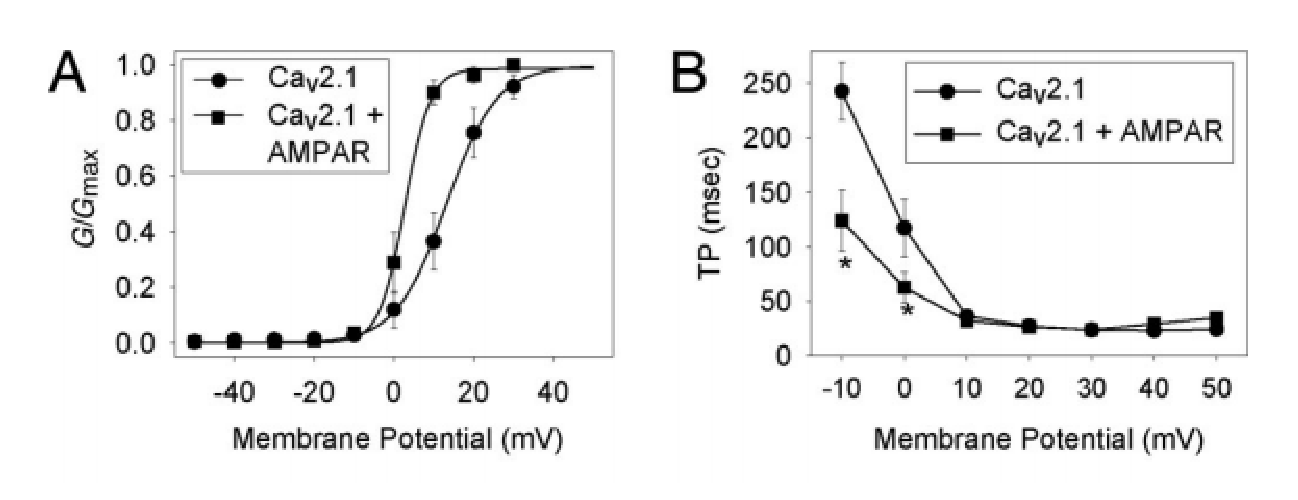
\includegraphics[height=5cm,
    angle=0]{./images/Cav2.1-AMPAR.eps}}
\caption{Cav2.1-AMPAR co-expression shift the activation of Cav2.1 to more
negative potential, and shorter time-to-peak \citep{kang2006}}
\label{fig:Cav2.1-AMPAR}
\end{figure}



\subsection{$\alpha$-isoform PSD-95 (SAP-90)}
\label{sec:PSD}

{\bf Postsynaptic density} (PSD) is a region central to the postsynaptic
membrane surface at which it is juxtaposed to the presynaptic membrane.
It is the place where NMDAR and/or AMPAR are typically anchored, via a
member of the MAGUK family, e.g. PSD-95 proteins or SAP97.

PSD-95 (postsynaptic densiqty protein 95) also known as SAP-90
(synapse-associated protein 90) is a protein (encoded by DLG4 gene) and is a 
member of the membrane-associated guanylate kinase (MAGUK) family
(Sect.\ref{sec:MAGUK}).

PSD-95 interacts: \url{https://en.wikipedia.org/wiki/DLG4}
\begin{itemize}
  \item 
\end{itemize}

\subsection{$\beta$-isoform SAP97}
\label{sec:SAP97}

SAP97 is a member of MAGUK family (Sect.\ref{sec:MAGUK}).
\begin{itemize}

  \item The L27 domain allows SAP97 to undergo oligamerization with other SAP97
molecules, as well as with the multi-domain scaffolding proteins containing L27
domains, such as CASK, Mint-1 and Velis.


  \item SAP97 possesses a myosin VI binding site  near the N-terminal.
SAP97 and  myosin VI are important for the endocytosis of GluR1-containing AMPA
receptors (Osterweil et al., 2005).
    
  \item  an alternatively spliced region between the SH3 and GK domains called
  the I3 region, a known binding site for the actin bindng protein protein 4.1N.
  
  Members of the  GKAP (Sect.\ref{sec:GKAP}) family of scaffolding proteins
  bind to the GK and SH3 domains of SAP97, facilitating its recruitment to the
  synapse (Thomas et al. 2000).

  I3 domain is involved in synaptic targ eting of SAP97, which results in an
  enlargement of the synaptic spine head along with an increase in surface
  expression of
GluR1-containing AMPA receptors at the synaptic surface, as well as increased
synaptic firing (Rumbaugh  et al. 2003)


\end{itemize}

In Parkinson diseases
\begin{enumerate}
  \item  GFP-tagged wild type SAP97 and SAP97 mutants were over-expressed in the
 striatum of 6-OHDA- lesioned rat model of Parkison disease (PD).
  
  A 19\% decrease in the total striatal content of SAP97 was reported in the 6-OHDA-
lesioned rat model of PD (Nash  et al.
 2005). Also, SAP97 is redistributed into the intracellular vesicular
 compartment.
  
  The levels of NR2B subunit in NMDAR of striatum is reduced.
  
   \item 
\end{enumerate}


\subsection{+ NMDAR, AMPAR (Glutamate release)}

A synapse either has GABAR or (NMDAR+AMPAR). They never on the same synapse.
NMDAR and AMPAR often \textcolor{red}{co-exist at the same (chemical) synapse of
the dendritic spines} (Sect.\ref{sec:dendritic_spines}). 

\begin{itemize}
  \item in Schaffer collateral-commissural (SCC) synapses of the adult rat:
  AMPAR and NMDAR colocalize on at least 75\% of synapses
  
  NMDAR:AMPAR current ratio is a linear function of PSD size
  (Sect.\ref{sec:PSD}), with AMPAR current drop to almost zero at PSD less than
  180nm. 
  
\end{itemize}

NMDAR and AMPAR are both glutamate receptors
(Sect.\ref{sec:glutamate_receptor}), i.e. they accept L-glutamate
(Sect.\ref{sec:Glutamate}) as ligands, but different subclass of each receptor
may requires co-binding of other ligands for activation, and their names come
from the specific synthetic subtance that are specific to their subclasss as the
ligand.

NMDAR and AMPAR have different physiological properties. Both are permeable to
$\Na$ (influx), and $\K$ (outward). These receptors have distinct kinetics
(AMPAR, 2-7 ms; NMDAR, 50-100 ms) and their contribution to EPSP are different
(Sect.\ref{sec:EPSP}).


The trafficking of AMPA receptors has also been suggested as one of the key
mechanisms for LTP and LTD. PSD95 or $\Ca$ channel $\gamma_2$ subunits
(stargazin) could be a candidate chaperon protein modulating AMPA receptor
trafficking depending on the $\Ca$ influx through $\Ca$ channels.

$\gamma_2$ subunit (stargazin) of neuronal $\Ca$ channels (Cav2.1, P/Q type)
were found to play a role in  the trafficking/clustering of AMPA receptors -
chaperon protein for proper folding and surface expression of AMPA receptors
(review: \citep{kang2006}). Stargazin also involves in the synaptic targeting of
AMPA receptors through its interaction with PSD95, a scaffolding protein
enriched in postsynaptic density (PSD).

\citep{kang2006} showed that native neuronal $\Ca$ channels can form a large
complex with postsynaptic proteins in the postsynaptic membrane and that this
association could change some biophysical properties of these $\Ca$ channels and
AMPA receptors.

\subsection{+ GABAR (GABA release)}

A synapse either has GABAR or (NMDAR+AMPAR). They never on the same synapse

Sect.\ref{sec:GABA_receptors}

\subsection{+ D1-receptor (Dopamine release)}

\subsection{+ D2-receptor (Dopamine release)}

\subsection{-- A2A receptor}
\label{sec:A2AReceptor-post-synaptic-side}

Adenosine A(2A) receptors (Sect.\ref{sec:A2A-receptor}) 
\begin{itemize}
  
  \item in striatum: A2AR are more concentrated in striatum than anywhere else
  in the brain, and preferentiallly localized in soma and dendrites of
  enkephalinergic-GABAergic-MSN (highly expressed D2-R, i.e. iSPN or D2-MSN -
  Sect.\ref{sec:D2-MSN}), but not dynorphinergic MSN, and 
  co-localized with D2 receptors .
  
  There was no enrichment of [(3)H]SCH 58261 binding or A(2A) receptor
  immunoreactivity in synaptosomal compared with total membranes from the
  striatum.
  
  They are found predominantly located in the postsynaptic density in the
  striatum (D2+ MSN) where they control the striatopallidal pathway thus
  controlling locomotion, although a minority of striatal A(2A) receptors were
  located in the presynaptic active zone

  
\end{itemize}

\subsection{SK channel}

In CA1 hippocampal neuron, synaptically evoked Ca(2+) influx through NMDARs
(Sect.\ref{sec:NMDAR}) activates spine SK channels, reducing EPSPs and the
associated spine head Ca(2+) transient.

\subsection{A-type Kv4.2 channel}

In CA1 hippocampal neuron, we also found Ca2+ influx via R-type Ca(2+) channels
(Cav2.3 - Sect.\ref{sec:Cav2.x}) to Kv4.2-containing channels.


 

\section{Both sides of synapses}
\label{sec:both-side-synapse}

\subsection{Mitochondria}

\url{http://www.cell.com/abstract/S0092-8674(04)01045-1}

\url{http://www.nature.com/nrn/journal/v6/n2/full/nrn1618.html}





\section{Drug agents}

\begin{itemize}
  \item PDE10 - Sect.\ref{sec:PDE10}
\end{itemize}

\section{Concentration detection of neurotransmitter}
\label{sec:glutamate-concentration-detection}

Methods for glutamate detection in intact cells are required, but classical
tools like microdialysis have suffered from low signal-to-noise ratios, poor
localization, and slow kinetics.


\section{Muscimol: THIP}
\label{sec:Muscimol}
\label{sec:THIP}

Muscimol can exist in two low-energy conformations: one conformation is
extended, while the other is partially folded. 

The conformationally restricted analogue to muscimol is 
4,5,6,7-tetrahydroisoxazolo[5,4-c]pyridin-3-ol (THIP).

In the case of THIP, there are also two low-energy conformations. However, both
of these exist in the partially folded conformation. The only difference between
the two conformations is the orientation of the nitrogen: in one conformation
the nitrogen is below and, in the other, the nitrogen is above the plane made by
THIP.
